\documentclass{article}\usepackage[]{graphicx}\usepackage[]{color}
%% maxwidth is the original width if it is less than linewidth
%% otherwise use linewidth (to make sure the graphics do not exceed the margin)
\makeatletter
\def\maxwidth{ %
  \ifdim\Gin@nat@width>\linewidth
    \linewidth
  \else
    \Gin@nat@width
  \fi
}
\makeatother

\definecolor{fgcolor}{rgb}{0.345, 0.345, 0.345}
\newcommand{\hlnum}[1]{\textcolor[rgb]{0.686,0.059,0.569}{#1}}%
\newcommand{\hlstr}[1]{\textcolor[rgb]{0.192,0.494,0.8}{#1}}%
\newcommand{\hlcom}[1]{\textcolor[rgb]{0.678,0.584,0.686}{\textit{#1}}}%
\newcommand{\hlopt}[1]{\textcolor[rgb]{0,0,0}{#1}}%
\newcommand{\hlstd}[1]{\textcolor[rgb]{0.345,0.345,0.345}{#1}}%
\newcommand{\hlkwa}[1]{\textcolor[rgb]{0.161,0.373,0.58}{\textbf{#1}}}%
\newcommand{\hlkwb}[1]{\textcolor[rgb]{0.69,0.353,0.396}{#1}}%
\newcommand{\hlkwc}[1]{\textcolor[rgb]{0.333,0.667,0.333}{#1}}%
\newcommand{\hlkwd}[1]{\textcolor[rgb]{0.737,0.353,0.396}{\textbf{#1}}}%

\usepackage{framed}
\makeatletter
\newenvironment{kframe}{%
 \def\at@end@of@kframe{}%
 \ifinner\ifhmode%
  \def\at@end@of@kframe{\end{minipage}}%
  \begin{minipage}{\columnwidth}%
 \fi\fi%
 \def\FrameCommand##1{\hskip\@totalleftmargin \hskip-\fboxsep
 \colorbox{shadecolor}{##1}\hskip-\fboxsep
     % There is no \\@totalrightmargin, so:
     \hskip-\linewidth \hskip-\@totalleftmargin \hskip\columnwidth}%
 \MakeFramed {\advance\hsize-\width
   \@totalleftmargin\z@ \linewidth\hsize
   \@setminipage}}%
 {\par\unskip\endMakeFramed%
 \at@end@of@kframe}
\makeatother

\definecolor{shadecolor}{rgb}{.97, .97, .97}
\definecolor{messagecolor}{rgb}{0, 0, 0}
\definecolor{warningcolor}{rgb}{1, 0, 1}
\definecolor{errorcolor}{rgb}{1, 0, 0}
\newenvironment{knitrout}{}{} % an empty environment to be redefined in TeX

\usepackage{alltt}

\usepackage{fancyhdr} % Required for custom headers
\usepackage{lastpage} % Required to determine the last page for the footer
\usepackage{extramarks} % Required for headers and footers
\usepackage{graphicx} % Required to insert images
\usepackage{hyperref}
\usepackage{amsmath} %for binomial pdf
\usepackage{parskip} % so that there's space bw paragraphs
\usepackage{float}
\usepackage{amsfonts}

% Margins
\topmargin=-0.45in
\evensidemargin=0in
\oddsidemargin=0in
\textwidth=6.5in
\textheight=9.0in
\headsep=0.25in 

\linespread{1.1} % Line spacing

% Set up the header and footer
\pagestyle{fancy}
\lhead{STAT 532: Bayes} % Top left header
\chead{HW 5} % Top center header
\rhead{Andrea Mack} % Top right header
\lfoot{10/31/2016} % Bottom left footer
\cfoot{} % Bottom center footer
\rfoot{Page\ \thepage\ of\ \pageref{LastPage}} % Bottom right footer
\renewcommand\headrulewidth{0.4pt} % Size of the header rule
\renewcommand\footrulewidth{0.4pt} % Size of the footer rule

\setlength\parindent{0pt} % Removes all indentation from paragraphs
\setlength\parskip{0.5cm}
\restylefloat{table}

%----------------------------------------------------------------------------------------
%	DOCUMENT STRUCTURE COMMANDS
%	Skip this unless you know what you're doing
%----------------------------------------------------------------------------------------

% Header and footer for when a page split occurs within a problem environment
\newcommand{\enterProblemHeader}[1]{
\nobreak\extramarks{#1}{#1 continued on next page\ldots}\nobreak
\nobreak\extramarks{#1 (continued)}{#1 continued on next page\ldots}\nobreak
}

% Header and footer for when a page split occurs between problem environments
\newcommand{\exitProblemHeader}[1]{
\nobreak\extramarks{#1 (continued)}{#1 continued on next page\ldots}\nobreak
\nobreak\extramarks{#1}{}\nobreak
}


%----------------------------------------------------------------------------------------%
\IfFileExists{upquote.sty}{\usepackage{upquote}}{}
\begin{document}


\begin{enumerate}
\item%1 
{\it (15 points) For this question we are going to take a deeper look at the impact of our prior
distributions and the number of observed data points. Generate fifteen observations from a
standard normal distribution and use independent priors on the parameters from the normal
distribution: p($\theta$) $\sim$ N($\mu_{o}$, $\tau_{o}^{2}$ ) and p($\sigma^2_{o}$) $\sim$ IG($\nu_{o}$/2, $\nu_{o}\simga^2_{o}$/2). This will require running the a Gibbs sampler to estimate the posterior distribution.

First plot the marginal posterior distributions for $\theta$ under the flat prior p($\theta$, $\sigma^2$) $\propto$ 1: Note that this is proportional to the likelihood function. }

{\normalfont Under the flat bivariate uniform prior on p($\theta,\sigma^2$), the marginal posterior on $\theta$ takes the form:}

$(2\pi)^{\frac{-(n+1)}{2}} * \Sigma(y_{i} - \theta)^{2}$ {\normalfont Using the observed sample of 15 $y_{i}$ and n = 15 from the standard normal distribution, the marginal posterior of $\theta$ is shown below. $\sigma^2$ is fixed to be 1.}


\begin{knitrout}
\definecolor{shadecolor}{rgb}{0.969, 0.969, 0.969}\color{fgcolor}

{\centering 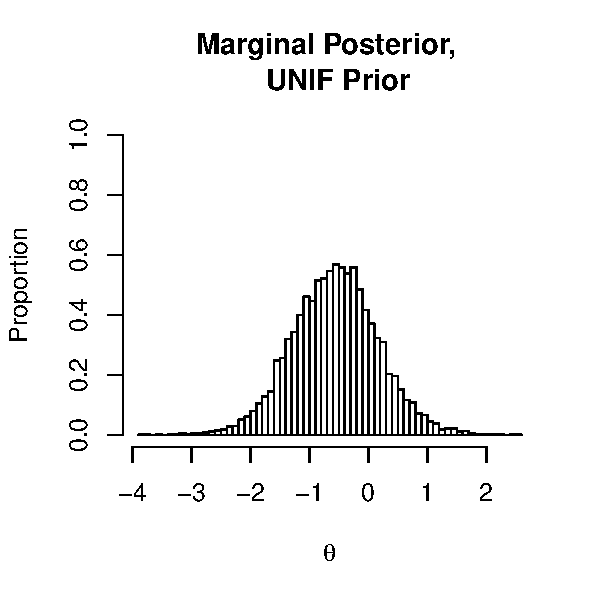
\includegraphics[width=\maxwidth]{figure/prob1-1} 

}



\end{knitrout}

{\it Next, rerun the Gibbs sampler using at least 5 different values for $\mu_{o}, \tau_{o}^2$ , where some of the values should be close to the truth and some should be very different. The same principles apply for $\sigma^2_{o}$, but fix p($\sigma^2_{o}$) $\propto \frac{1}{\sigma^2}$ so that we can see the difference for $\theta$. Make sure to look at a few situations where $\tau_{o}^2$ is very small and very large. Explain what you have learned from this question and create a figure that contains the prior, likelihood, and posterior on a single graph.}

\begin{knitrout}
\definecolor{shadecolor}{rgb}{0.969, 0.969, 0.969}\color{fgcolor}

{\centering 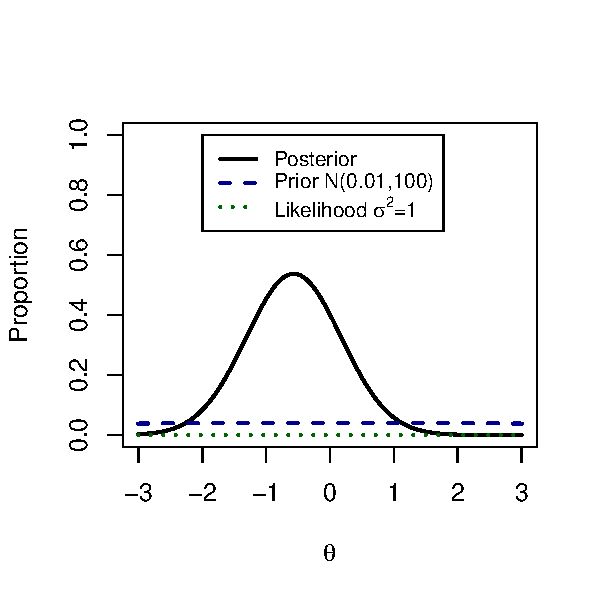
\includegraphics[width=\maxwidth]{figure/prob1x-1} 

}



\end{knitrout}


\begin{knitrout}
\definecolor{shadecolor}{rgb}{0.969, 0.969, 0.969}\color{fgcolor}
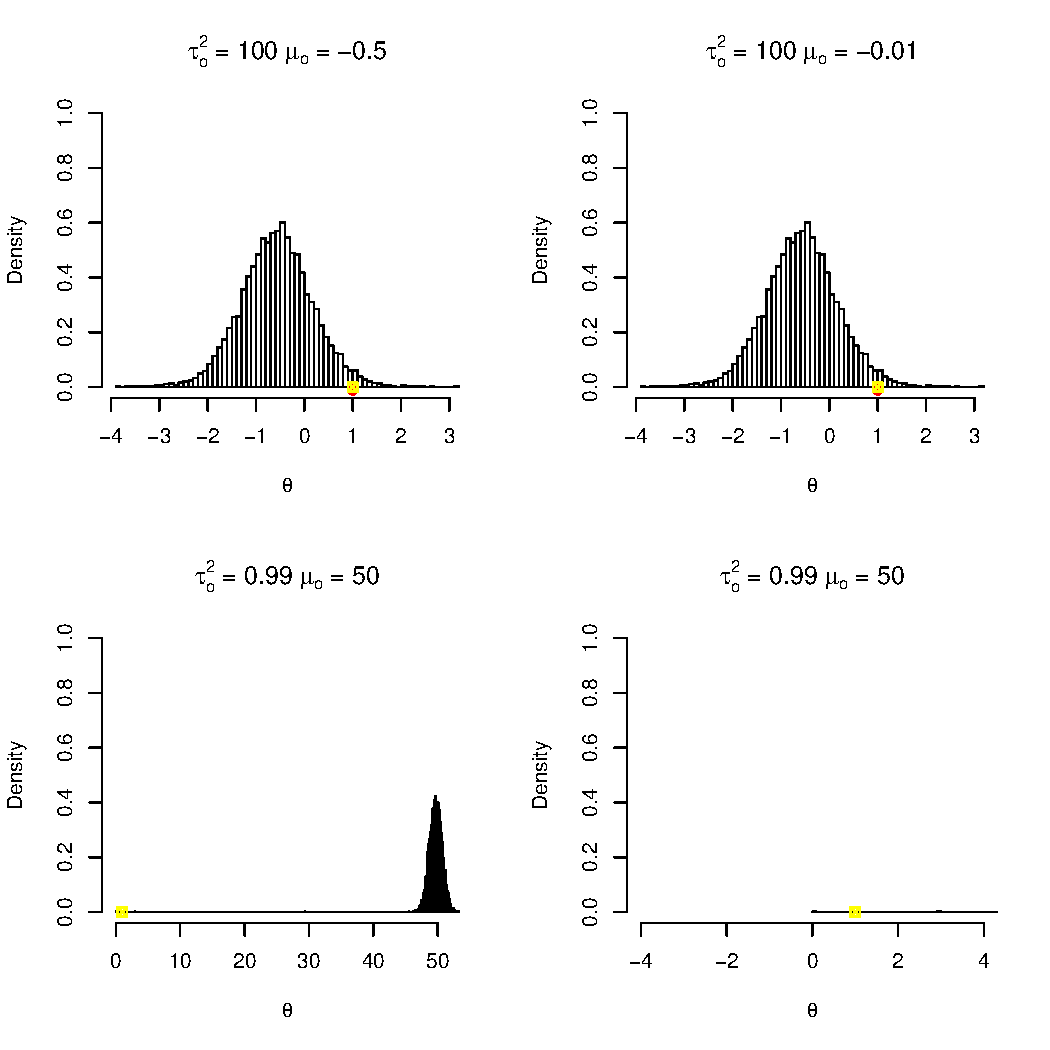
\includegraphics[width=\maxwidth]{figure/prob1xxx-1} 

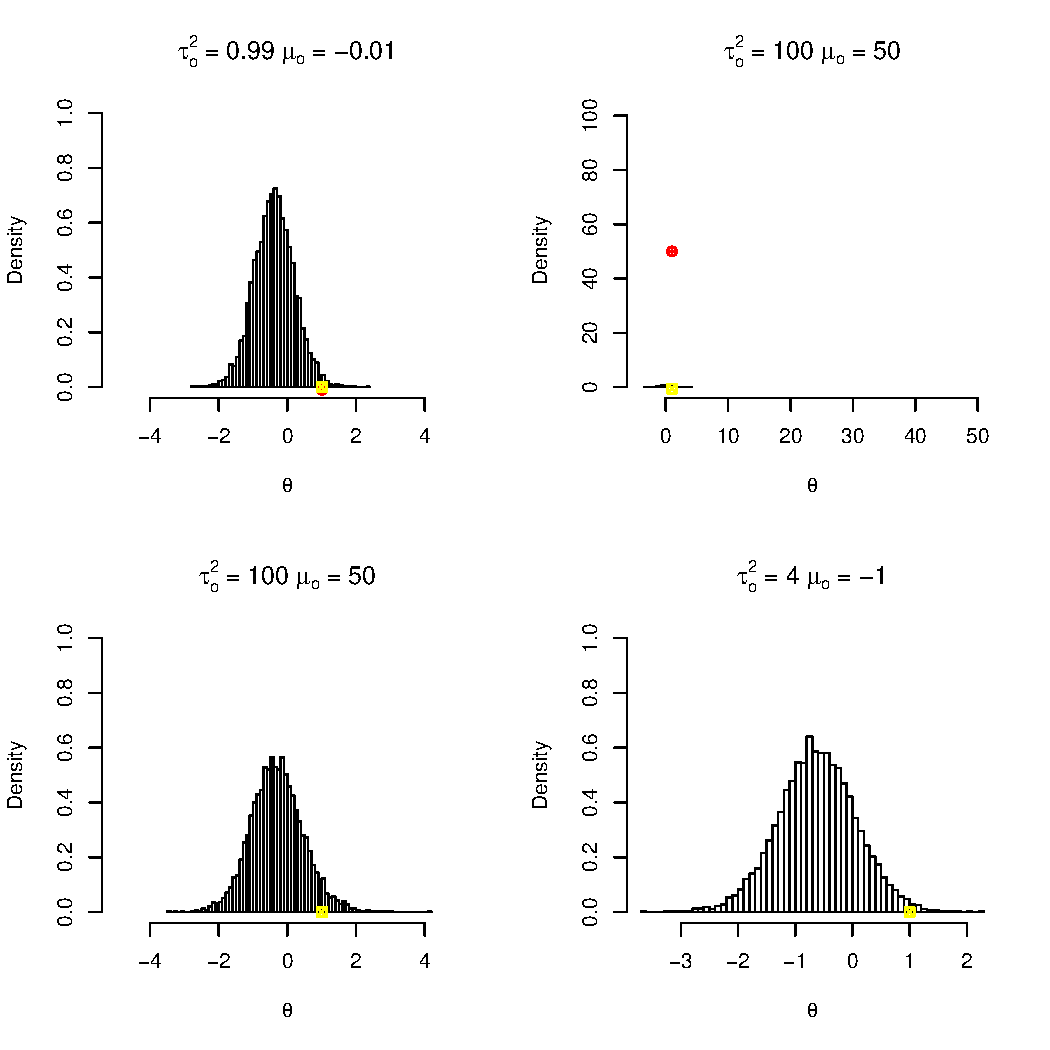
\includegraphics[width=\maxwidth]{figure/prob1xxx-2} 

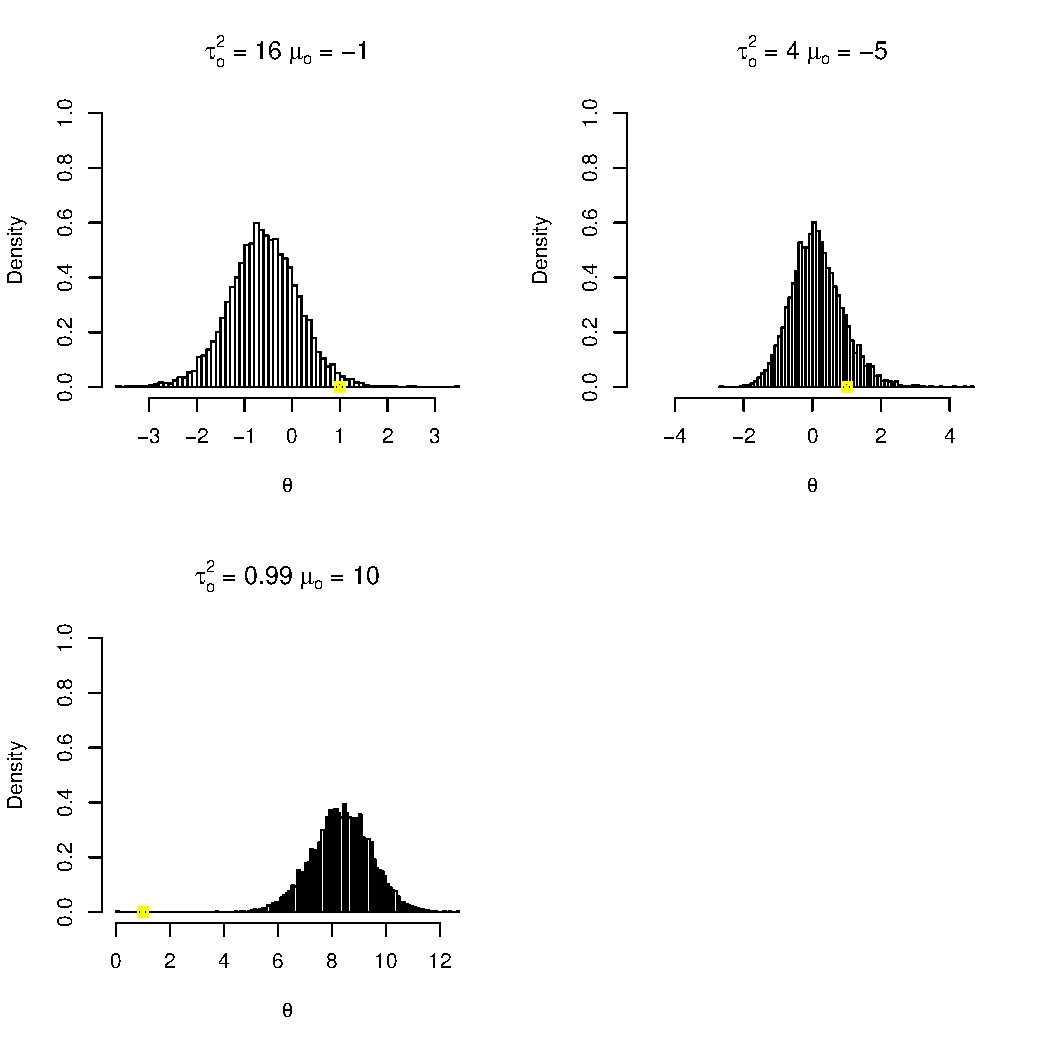
\includegraphics[width=\maxwidth]{figure/prob1xxx-3} 

\end{knitrout}


The axes may change. In each plot, the red represents the initializations of $\mu_{o}$ and $\tau_{o}$ and the yellow represents the true mean and variance of the 15 simulated points from the standard normal distribution where how close the two initializations are to the truth varied. Note that $\tau_{o}^2$ is not $\sigma^2$ since $\tau_{o}^2 = \frac{\sigma^2}{\kappa_{o}}$, and neither are not plotted.

If $\tau_{o}^2$ is somewhat far from the truth, the marginal posterior of $\theta$ is generally unbiased. However, if not, then the marginal posterior of $\theta$ is centered near the initialized $\mu_{o}$. The spread appears to be robust for all initializations of $\tau_{o}^2$.

\item {\it (10 points) Assume you are faced with a modeling scenario for a multivariate normal response where you do not have a good sense of the covariance structure. Select and justify a prior distribution for $\Sigma$ of ($\Sigma^{-1}$).}

Generally the gamma distribution is used as a prior on the precision parameter in the univariate normal case. The Wishart distribution is a multivariate form of the gamma distribution, and so makes sense for the prior on the multivariate covariance matrix, $\Sigma$. 

The prior on $\Sigma$  requires parameters, $\nu_{o}$ and $\Psi_{o}$. Let p = the number of groups in the multivariate normal distribution. Choose $\nu_{o}$ = p+2 to make the prior less informative as the E[$\Sigma$] = $\frac{1}{\nu_{o} - p - 1}*S_{o}$ = $S_{o}$. Note $\nu_{o}$ can be thought of as the prior sample size, and we need at least one observation per group, so setting $\nu_{o}$ this ways would mean we have very little information, nearly one observation, in each group.

$S_{o}$ is the prior sums of squares. In class, choosing the off-diagonal elements to be 0 was less restrictive than assuming non-zero covariance terms between observations. Setting the diagonal elements to 100 is fairly nonrestrictive as it allows for enough variation to make the prior have more spread and therefore be less informative.

\item {\it (10 points) Verify that for a multivariate normal distribution, the variance and expectation can be extracted from the kernel, exp[$\frac{-1}{2}(\widetilde{\theta^{t}}A\widetilde{\theta} - \widetilde{\theta^{t}}B + ...)]$, where the variance is $A^{-1}$ and the expectation is $A^{-1}B$.}

The kernal of a multivariate distribution of $\widtilde{\theta} | A, B$ is given in the problem description. Consider exp[$\phi$] = exp[$\frac{-1}{2}(\widetilde{\theta^{t}}A\widetilde{\theta} - \widetilde{\theta^{t}}B + ...)] \ni 

$\phi =  -\frac{1}{2} \widetilde{\theta^{t}}A\widetilde{\theta} - \widetilde{\theta^{t}}B + ....$


$\propto -\frac{1}{2} (A^{-1})^{-1} (\widetilde{\theta}^{T}\widetilde{\theta} - \widetilde{\theta}^{T}A^{-1}B - c\widetilde{\theta})$ from p.58 in the notes

$\propto -\frac{1}{2} (A^{-1})^{-1} (\widetilde{\theta}^{T}\widetilde{\theta} - \widetilde{\theta}^{T}A^{-1}B - \widetilde{\theta}^{T}c)$ c is symmetric

$\propto -\frac{1}{2} (A^{-1})^{-1} (\widetilde{\theta}^{T}\widetilde{\theta} - 2\widetilde{\theta}^{T}A^{-1}B)$

$\propto -\frac{1}{2} (A^{-1})^{-1} (\widetilde{\theta}^{T}\widetilde{\theta} - 2\widetilde{\theta}^{T}A^{-1}B + (A^{-1}B)^{T}(A^{-1}B)) + \frac{1}{2} (A^{-1})^{-1}(A^{-1}B)^{T}(A^{-1}B)$

$\propto -\frac{1}{2} (A^{-1})^{-1} (\widetilde{\theta}^{T} - (A^{-1}B)^{T})(\widetilde{\theta} - (A^{-1}B))$

$\propto -\frac{1}{2} [((\widetilde{\theta} - (A^{-1}B))^{T})(A^{-1})^{-1} (\widetilde{\theta} - (A^{-1}B))]$

\rightarrow E[$\widetilde{\theta}$] = ($A^{-1}B$); Var[$\widetilde{\theta}] = A^{-1}$

\item %4
{\it (20 points) Simulate data from a multivariate normal distribution, with p = 3. Choose a mean vector mu and covariance matrix sigma. Run a Gibbs sampler and verify that your sampler returns the true values. Comment on the results.}

The true expected value in all groups is 0 and the true correlation matrix is the identity matrix. The prior means on $\widetilde{\theta}$ were all 0 and the prior covariance matrix was fairly uninformative as diag(100). The prior sample size for $\Sigma$ must be at least p = the number of groups = 3. Making the prior sample size small makes the prior less informative, let the prior sample size be 5 for all groups. Set the prior residual sums of squares matrix to be diag(10) which is uninformative relative to the prior means.
\begin{knitrout}
\definecolor{shadecolor}{rgb}{0.969, 0.969, 0.969}\color{fgcolor}

{\centering 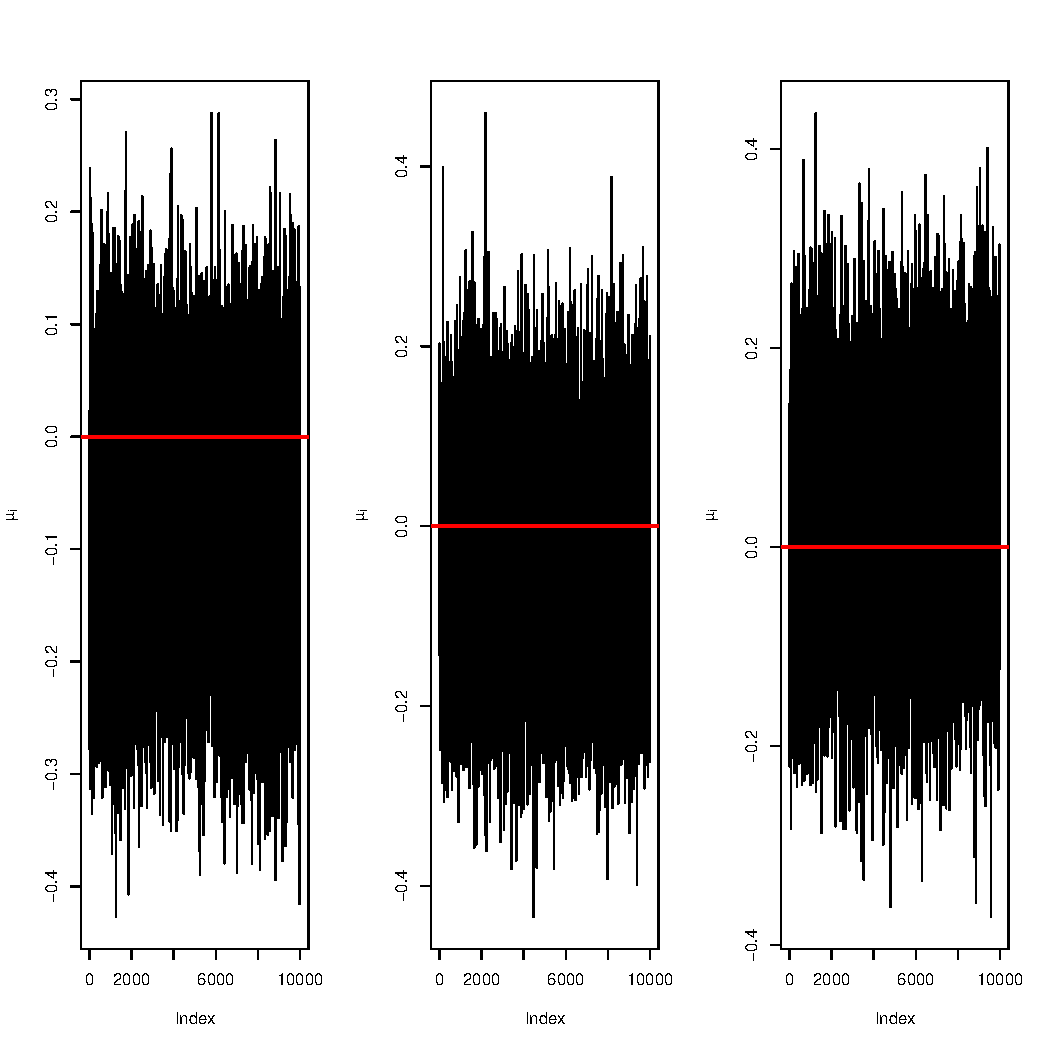
\includegraphics[width=\maxwidth]{figure/prob4-1} 

}



\end{knitrout}

\begin{knitrout}
\definecolor{shadecolor}{rgb}{0.969, 0.969, 0.969}\color{fgcolor}
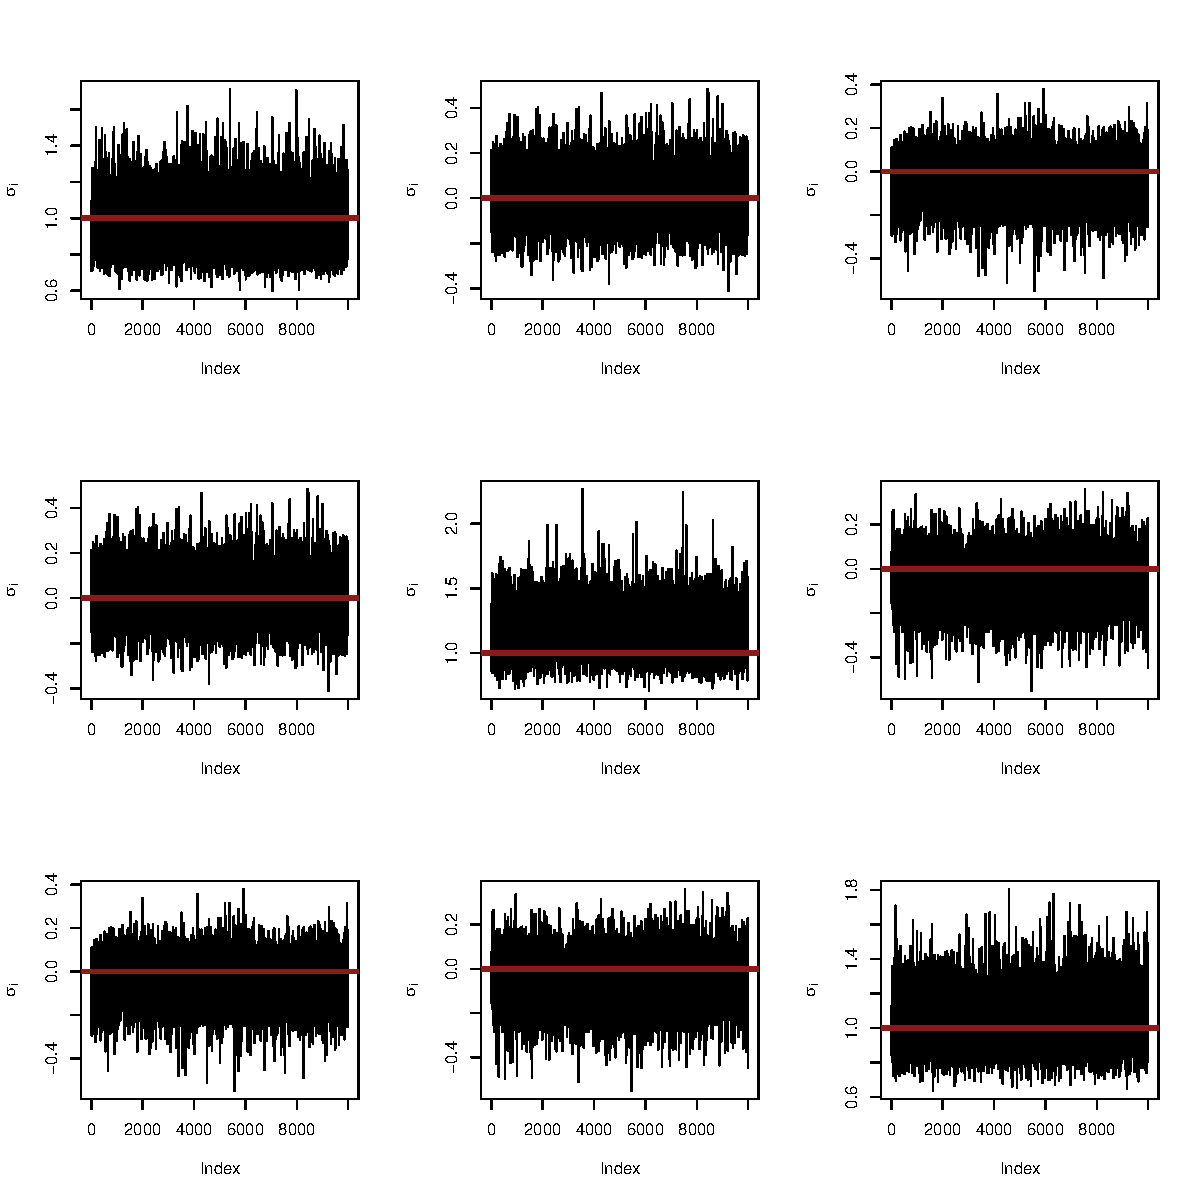
\includegraphics[width=\maxwidth]{figure/prob4x-1} 

\end{knitrout}

The trace plots for the posterior on $\widetilde{\theta}$ show unbiased convergence to the true mean, 0, quite fast which was to be expected because both the true means for the random draws and the prior means were set to 0. By making the posteriors fairly uniformative, we see unbiased convergence of the posterior on $\widetilde{\sigma}^2$ to the prior correlation matrix (the identity) quickly as well which is seen in the diagonal plots being centered at 1 and the off diagonal trace plots being centered at 0.


\item {\it Modeling heavy tailed distributions}.

\begin{enumerate}
\item

y $\sim$ N($\theta, \sigma^2 * \gamma$) 

$\sigma^2 \sim$ IG(a,b)

Find p(y $| \theta,\gamma$) = $\int p(y | \theta,\gamma,\sigma^2)p(\sigma^2)d\sigma^2$

\propto $\int (\sigma^{2}\gamma\pi)^{-1/2}exp[\frac{-1}{2\sigma^{2}\gamma}(y-\theta)^{2}]\frac{(\frac{1}{\sigma^{2}})^{a - 1}exp[\frac{-1}{\sigma^2}b]b^{a}}{\Gamma(a)}d\sigma^{2}$

\propto $ (\pi\gamma)^{-1/2}*\frac{b^{a}}{\Gamma(a)} \int (\frac{1}{\sigma^{2}})^{a + \frac{1}{2} - 1} exp[\frac{-1}{\sigma^2}(\frac{(y-\theta)^{2}}{2\gamma} + b)]d\sigma^{2}$

\propto $ (\pi\gamma)^{-1/2}\Gamma(a + \frac{1}{2})*\frac{b^{a}}{\Gamma(a)*[\frac{(y-\theta)^{2}}{2\gamma} + b]^{a+\frac{1}{2}}} * 1.$

This is because we get out a GAM(a+$\frac{1}{2}, \frac{(y-\theta)^{2}}{2\gamma} + b$)

Let a = $\frac{1}{2}$ and b = 1:

\propto $(\pi\gamma)^{-1/2}\Gamma(\frac{1}{2} + \frac{1}{2})*\frac{1}{\Gamma(\frac{1}{2})*[\frac{(y-\theta)^{2}}{2\gamma} + 1]^{1}}$

\propto $(\gamma)^{-1/2}*\frac{1}{\pi}*\frac{1}{[\frac{(y-\theta)^{2}}{2\gamma} + 1]}$

The above is not in the correct form. Now let a = $\frac{1}{2}$ and b = $\frac{1}{2}$:

\propto $(\pi\gamma)^{-1/2}\Gamma(\frac{1}{2} + \frac{1}{2})*\frac{1}{\Gamma(\frac{1}{2})*[\frac{(y-\theta)^{2}}{2\gamma} + \frac{1}{2}]^{1}2^{\frac{1}{2}}}$

\propto $2*(\gamma)^{-1/2}*\frac{1}{\pi}*\frac{1}{[\frac{(y-\theta)^{2}}{\gamma} + 1]2^{\frac{1}{2}}}$

\propto $(\gamma)^{-1/2}*\frac{1}{\pi}*\frac{1}{[\frac{(y-\theta)^{2}}{\gamma} + 1]}$

This shows p(y$|\theta, \gamma$) \propto Cauchy($\theta$, variance = $\gamma$).

\item 
The location is $\theta$ and the scale is actually the standard deviation, so $\gamma^{\frac{1}{2}}$ which holds when a = $\frac{1}{2}$ and b = $\frac{1}{2}$.

\item {\it Generate a posterior predictive distribution for $y^{*}$.}

I assumed we were supposed to fix $\gamma$ and $\theta$, so that p($\lambda$) = p($\sigma^2$) and p(y $| \lambda^{*}$) = p(y $| \gamma, \theta, \sigma^2$) where $\gamma$ and $\theta$ are somewhat arbitrarily chosen to be fixed at 2 and 0, respectively.

In parts (a) and (b) we showed that if a = $\frac{1}{2}$ and b = $\frac{1}{2}$, then p(y $| \theta, \gamma$) is Cauchy($\theta, \gamma$). Use these values for the prior on $\sigma^2$ and generate $y^{*}$ from a N(0,2$\sigma^2$) distribution where each $\sigma^2$ is drawn independently.

\begin{knitrout}
\definecolor{shadecolor}{rgb}{0.969, 0.969, 0.969}\color{fgcolor}

{\centering 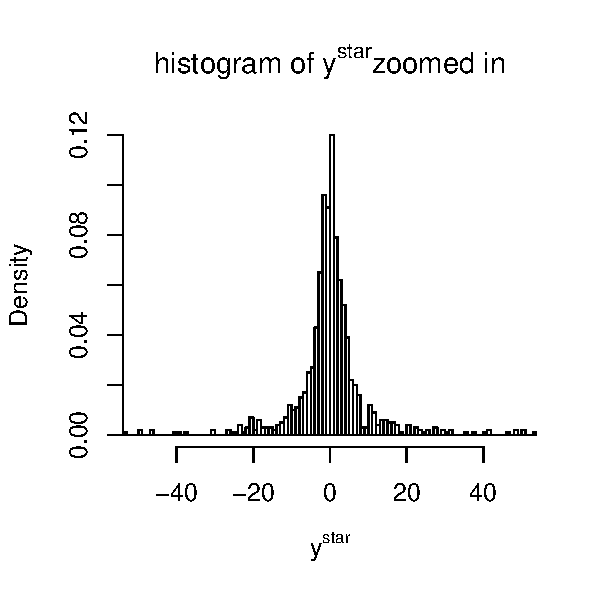
\includegraphics[width=\maxwidth]{figure/prob5c-1} 

}




{\centering 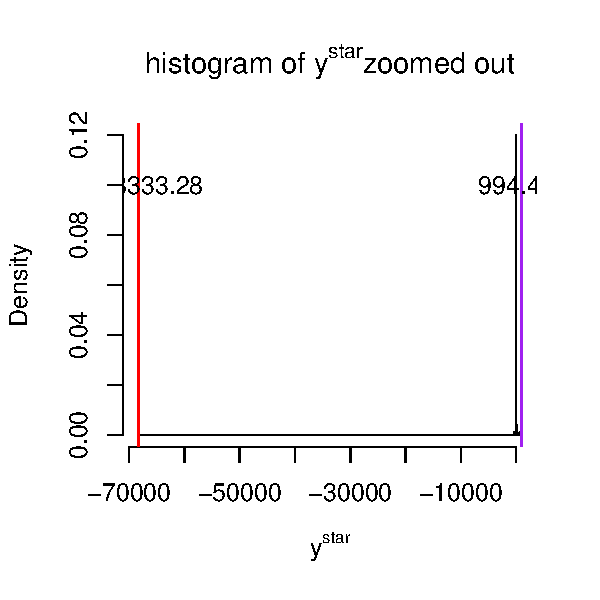
\includegraphics[width=\maxwidth]{figure/prob5c-2} 

}




{\centering 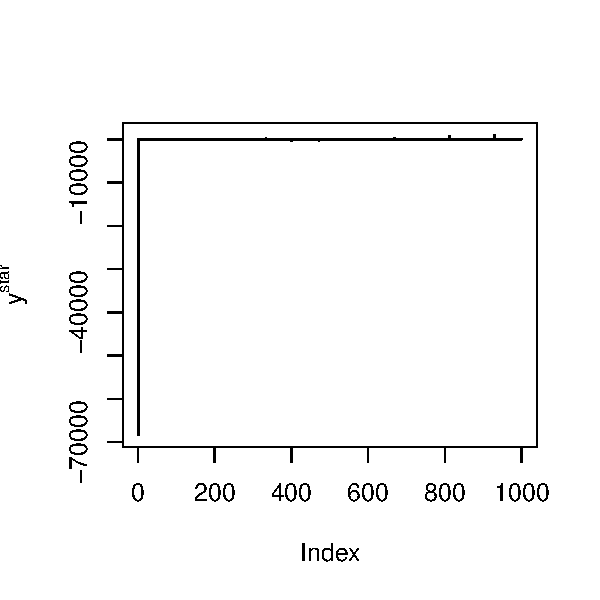
\includegraphics[width=\maxwidth]{figure/prob5c-3} 

}




{\centering 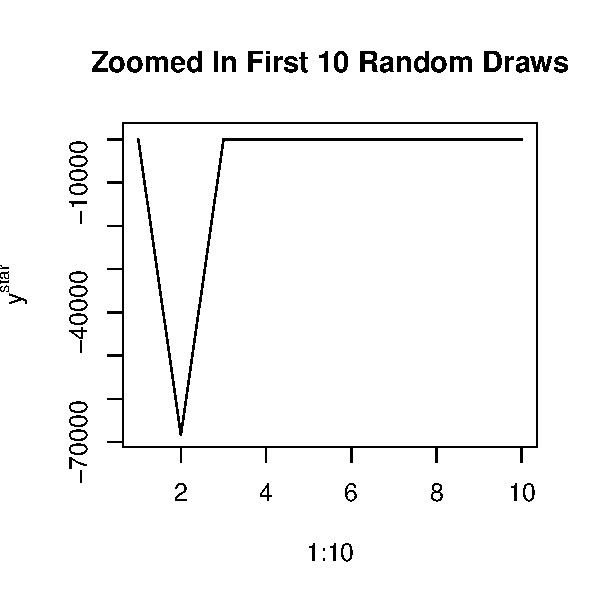
\includegraphics[width=\maxwidth]{figure/prob5c-4} 

}



\end{knitrout}

Zooming in we see the majority of the mass of p($y^{*} | \theta, \gamma$) forms a symmetric distribution about 0. There was an outlier in the draws for the precision term, making the histogram of all observations not helpful. Zooming in, p($y^{*} | \theta, \gamma$), is still quite dispersed.

\item In the context of modeling over-dispersed data, $\gamma$ can be set to a fractional number, making thicker tails in the normal distribution. The distribution is still a bell-shaped curve, but with more observations in the tails. The result that the posterior predictive distribution is Cauchy is useful because it is easy to sample from.

In terms of modeling over-dispersed data, the result is useful because we only need to set values of $\theta$ and $\gamma$, the mean and over-dispersion parameters and the prior on $\sigma^2$ is always the same.

\end{enumerate}

\item 

I will choose to read {\it Bayesian Geostatistical Design} by Diggle and Lophaven.

For the project, what will we need to be included in the summary of our work?

\end{enumerate}

\section*{R Code}
\begin{enumerate}
{\tiny
\item 
\begin{knitrout}
\definecolor{shadecolor}{rgb}{0.969, 0.969, 0.969}\color{fgcolor}\begin{kframe}
\begin{alltt}
\hlcom{#draw randomly from stand norm 15 observations}

\hlkwd{set.seed}\hlstd{(}\hlnum{53205}\hlstd{)}
\hlstd{y15} \hlkwb{<-} \hlkwd{rnorm}\hlstd{(}\hlnum{15}\hlstd{,}\hlnum{0}\hlstd{,}\hlnum{1}\hlstd{)}

\hlcom{#simulate the joint posterior}
\hlstd{num.sims} \hlkwb{<-} \hlnum{10000}
\hlstd{Phi} \hlkwb{<-} \hlkwd{matrix}\hlstd{(}\hlnum{0}\hlstd{,}\hlkwc{nrow}\hlstd{=num.sims,}\hlkwc{ncol}\hlstd{=}\hlnum{2}\hlstd{)}
\hlstd{Phi[}\hlnum{1}\hlstd{,}\hlnum{1}\hlstd{]} \hlkwb{<-} \hlnum{0} \hlcom{# initialize theta}
\hlstd{Phi[}\hlnum{1}\hlstd{,}\hlnum{2}\hlstd{]} \hlkwb{<-} \hlnum{1} \hlcom{# initialize (1/sigmasq)}
\hlstd{mu.0} \hlkwb{<-} \hlnum{0}
\hlstd{tausq.0} \hlkwb{<-} \hlnum{100}
\hlstd{nu.0} \hlkwb{<-} \hlnum{1}
\hlstd{sigmasq.0} \hlkwb{<-} \hlnum{100}
\hlstd{num.obs} \hlkwb{<-} \hlkwd{length}\hlstd{(y15)}

\hlstd{mean.y} \hlkwb{<-} \hlkwd{mean}\hlstd{(y15)}

\hlkwa{for} \hlstd{(i} \hlkwa{in} \hlnum{2}\hlopt{:}\hlstd{num.sims)\{}
  \hlcom{# sample theta from full conditional}
  \hlstd{mu.n} \hlkwb{<-} \hlstd{(mu.0} \hlopt{/} \hlstd{tausq.0} \hlopt{+} \hlstd{num.obs} \hlopt{*} \hlstd{mean.y} \hlopt{*}\hlstd{Phi[(i}\hlopt{-}\hlnum{1}\hlstd{),}\hlnum{2}\hlstd{])} \hlopt{/} \hlstd{(}\hlnum{1} \hlopt{/} \hlstd{tausq.0} \hlopt{+} \hlstd{num.obs} \hlopt{*} \hlstd{Phi[(i}\hlopt{-}\hlnum{1}\hlstd{),}\hlnum{2}\hlstd{] )}
  \hlstd{tausq.n} \hlkwb{<-} \hlnum{1} \hlopt{/} \hlstd{(}\hlnum{1}\hlopt{/}\hlstd{tausq.0} \hlopt{+} \hlstd{num.obs} \hlopt{*} \hlstd{Phi[(i}\hlopt{-}\hlnum{1}\hlstd{),}\hlnum{2}\hlstd{])}
  \hlstd{Phi[i,}\hlnum{1}\hlstd{]} \hlkwb{<-} \hlkwd{rnorm}\hlstd{(}\hlnum{1}\hlstd{,mu.n,}\hlkwd{sqrt}\hlstd{(tausq.n))}

  \hlcom{# sample (1/sigma.sq) from full conditional}
  \hlstd{nu.n} \hlkwb{<-} \hlstd{nu.0} \hlopt{+} \hlstd{num.obs}
  \hlstd{sigmasq.n.theta} \hlkwb{<-} \hlnum{1}\hlopt{/}\hlstd{nu.n}\hlopt{*}\hlstd{(nu.0}\hlopt{*}\hlstd{sigmasq.0} \hlopt{+} \hlkwd{sum}\hlstd{((y15} \hlopt{-} \hlstd{Phi[i,}\hlnum{1}\hlstd{])}\hlopt{^}\hlnum{2}\hlstd{))}
  \hlstd{Phi[i,}\hlnum{2}\hlstd{]} \hlkwb{<-} \hlkwd{rgamma}\hlstd{(}\hlnum{1}\hlstd{,nu.n}\hlopt{/}\hlnum{2}\hlstd{,nu.n}\hlopt{*}\hlstd{sigmasq.n.theta}\hlopt{/}\hlnum{2}\hlstd{)}
\hlstd{\}}
\hlcom{## first figure out what the "truth" is for my simulations}
\hlcom{## although not really necessary, truth = 0,1}
\hlstd{y15.true.mean} \hlkwb{<-} \hlkwd{mean}\hlstd{(y15)}
\hlstd{y15.true.var} \hlkwb{<-} \hlkwd{var}\hlstd{(y15)}

\hlkwd{par}\hlstd{(}\hlkwc{mfrow} \hlstd{=} \hlkwd{c}\hlstd{(}\hlnum{1}\hlstd{,}\hlnum{1}\hlstd{))}
\hlkwd{hist}\hlstd{(Phi[,}\hlnum{1}\hlstd{],} \hlkwc{freq} \hlstd{=} \hlnum{FALSE}\hlstd{,} \hlkwc{breaks} \hlstd{=} \hlstr{"fd"}\hlstd{,} \hlkwc{xlab} \hlstd{=} \hlkwd{expression}\hlstd{(theta),} \hlkwc{ylab} \hlstd{=} \hlstr{"Proportion"}\hlstd{,} \hlkwc{main} \hlstd{=} \hlstr{"Marginal Posterior, \textbackslash{}n  UNIF Prior"}\hlstd{,} \hlkwc{ylim}\hlstd{=}\hlkwd{c}\hlstd{(}\hlnum{0}\hlstd{,}\hlnum{1}\hlstd{))}


\hlcom{## generating from bivariate uniform}
\hlcom{## since theta and sigma2 are orthogonal, generate two observations randomly from unif(0,1)}
\end{alltt}
\end{kframe}
\end{knitrout}
\begin{knitrout}
\definecolor{shadecolor}{rgb}{0.969, 0.969, 0.969}\color{fgcolor}\begin{kframe}
\begin{alltt}
\hlcom{## rerun for several different values of mu.o and tau.o}


\hlcom{## 1 close mean, far var}

\hlcom{#simulate the joint posterior}
\hlstd{num.sims} \hlkwb{<-} \hlnum{10000}
\hlstd{Phi} \hlkwb{<-} \hlkwd{matrix}\hlstd{(}\hlnum{0}\hlstd{,}\hlkwc{nrow}\hlstd{=num.sims,}\hlkwc{ncol}\hlstd{=}\hlnum{2}\hlstd{)}
\hlstd{Phi[}\hlnum{1}\hlstd{,}\hlnum{1}\hlstd{]} \hlkwb{<-} \hlnum{0} \hlcom{# initialize theta}
\hlstd{Phi[}\hlnum{1}\hlstd{,}\hlnum{2}\hlstd{]} \hlkwb{<-} \hlnum{1} \hlcom{# initialize (1/sigmasq)}
\hlstd{mu.0} \hlkwb{<-} \hlopt{-}\hlnum{0.01}
\hlstd{tausq.0} \hlkwb{<-} \hlnum{100}
\hlstd{nu.0} \hlkwb{<-} \hlnum{1}
\hlstd{sigmasq.0} \hlkwb{<-} \hlnum{100}
\hlstd{num.obs} \hlkwb{<-} \hlkwd{length}\hlstd{(y15)}

\hlstd{mean.y} \hlkwb{<-} \hlkwd{mean}\hlstd{(y15)}

\hlkwa{for} \hlstd{(i} \hlkwa{in} \hlnum{2}\hlopt{:}\hlstd{num.sims)\{}
  \hlcom{# sample theta from full conditional}
  \hlstd{mu.n} \hlkwb{<-} \hlstd{(mu.0} \hlopt{/} \hlstd{tausq.0} \hlopt{+} \hlstd{num.obs} \hlopt{*} \hlstd{mean.y} \hlopt{*}\hlstd{Phi[(i}\hlopt{-}\hlnum{1}\hlstd{),}\hlnum{2}\hlstd{])} \hlopt{/} \hlstd{(}\hlnum{1} \hlopt{/} \hlstd{tausq.0} \hlopt{+} \hlstd{num.obs} \hlopt{*} \hlstd{Phi[(i}\hlopt{-}\hlnum{1}\hlstd{),}\hlnum{2}\hlstd{] )}
  \hlstd{tausq.n} \hlkwb{<-} \hlnum{1} \hlopt{/} \hlstd{(}\hlnum{1}\hlopt{/}\hlstd{tausq.0} \hlopt{+} \hlstd{num.obs} \hlopt{*} \hlstd{Phi[(i}\hlopt{-}\hlnum{1}\hlstd{),}\hlnum{2}\hlstd{])}
  \hlstd{Phi[i,}\hlnum{1}\hlstd{]} \hlkwb{<-} \hlkwd{rnorm}\hlstd{(}\hlnum{1}\hlstd{,mu.n,}\hlkwd{sqrt}\hlstd{(tausq.n))}

  \hlcom{# sample (1/sigma.sq) from full conditional}
  \hlstd{nu.n} \hlkwb{<-} \hlstd{nu.0} \hlopt{+} \hlstd{num.obs}
  \hlstd{sigmasq.n.theta} \hlkwb{<-} \hlnum{1}\hlopt{/}\hlstd{nu.n}\hlopt{*}\hlstd{(nu.0}\hlopt{*}\hlstd{sigmasq.0} \hlopt{+} \hlkwd{sum}\hlstd{((y15} \hlopt{-} \hlstd{Phi[i,}\hlnum{1}\hlstd{])}\hlopt{^}\hlnum{2}\hlstd{))}
  \hlstd{Phi[i,}\hlnum{2}\hlstd{]} \hlkwb{<-} \hlkwd{rgamma}\hlstd{(}\hlnum{1}\hlstd{,nu.n}\hlopt{/}\hlnum{2}\hlstd{,nu.n}\hlopt{*}\hlstd{sigmasq.n.theta}\hlopt{/}\hlnum{2}\hlstd{)}
\hlstd{\}}

\hlkwd{par}\hlstd{(}\hlkwc{mfrow}\hlstd{=}\hlkwd{c}\hlstd{(}\hlnum{1}\hlstd{,}\hlnum{1}\hlstd{))}
\hlcom{#plot prior, posterior, and likelihood}
\hlstd{post.x} \hlkwb{<-} \hlkwa{function}\hlstd{(}\hlkwc{x}\hlstd{)\{}\hlnum{2}\hlopt{*}\hlstd{pi}\hlopt{^}\hlstd{((}\hlopt{-}\hlkwd{length}\hlstd{(y15))}\hlopt{/}\hlnum{2}\hlstd{)}\hlopt{*}\hlkwd{exp}\hlstd{(}\hlopt{-}\hlstd{((}\hlkwd{sum}\hlstd{(y15)}\hlopt{^}\hlnum{2}\hlstd{)} \hlopt{+} \hlnum{2}\hlopt{*}\hlkwd{sum}\hlstd{(y15)}\hlopt{*}\hlstd{x} \hlopt{-}\hlstd{x}\hlopt{^}\hlnum{2}\hlstd{)}\hlopt{/}\hlnum{2}\hlstd{)\}}

\hlkwd{curve}\hlstd{(}\hlkwd{dnorm}\hlstd{(x,} \hlkwc{mean} \hlstd{=} \hlkwd{mean}\hlstd{(Phi[,}\hlnum{1}\hlstd{]),} \hlkwc{sd} \hlstd{=} \hlkwd{sqrt}\hlstd{(}\hlkwd{var}\hlstd{(Phi[,}\hlnum{1}\hlstd{]))),} \hlkwc{ylim} \hlstd{=} \hlkwd{c}\hlstd{(}\hlnum{0}\hlstd{,}\hlnum{1}\hlstd{),} \hlkwc{xlim} \hlstd{=} \hlkwd{c}\hlstd{(}\hlopt{-}\hlnum{3}\hlstd{,}\hlnum{3}\hlstd{),}\hlkwc{lwd} \hlstd{=} \hlnum{2}\hlstd{,} \hlkwc{xlab} \hlstd{=} \hlkwd{expression}\hlstd{(theta),} \hlkwc{ylab} \hlstd{=} \hlstr{"Proportion"}\hlstd{,} \hlkwc{lty} \hlstd{=} \hlnum{1}\hlstd{)}
\hlkwd{curve}\hlstd{(}\hlkwd{dnorm}\hlstd{(x,} \hlkwc{mean}\hlstd{=}\hlnum{0}\hlstd{,} \hlkwc{sd}\hlstd{=}\hlnum{10}\hlstd{),}
          \hlkwc{col}\hlstd{=}\hlstr{"darkblue"}\hlstd{,} \hlkwc{lwd}\hlstd{=}\hlnum{2}\hlstd{,} \hlkwc{add}\hlstd{=}\hlnum{TRUE}\hlstd{,} \hlkwc{yaxt}\hlstd{=}\hlstr{"n"}\hlstd{,} \hlkwc{lty} \hlstd{=} \hlnum{2}\hlstd{)}
\hlkwd{curve}\hlstd{(post.x,} \hlkwc{col}\hlstd{=}\hlstr{"darkgreen"}\hlstd{,} \hlkwc{lwd}\hlstd{=}\hlnum{2}\hlstd{,} \hlkwc{add}\hlstd{=}\hlnum{TRUE}\hlstd{,} \hlkwc{yaxt}\hlstd{=}\hlstr{"n"}\hlstd{,} \hlkwc{lty} \hlstd{=} \hlnum{3}\hlstd{)}
\hlkwd{legend}\hlstd{(}\hlopt{-}\hlnum{2}\hlstd{,}\hlnum{1}\hlstd{,} \hlkwc{legend} \hlstd{=} \hlkwd{c}\hlstd{(}\hlstr{"Posterior"}\hlstd{,} \hlstr{"Prior N(0.01,100)"}\hlstd{,} \hlkwd{expression}\hlstd{(}\hlkwd{paste}\hlstd{(}\hlstr{"Likelihood "}\hlstd{, sigma}\hlopt{^}\hlnum{2}\hlstd{,} \hlstr{"=1"}\hlstd{))),}\hlkwc{lty}\hlstd{=}\hlkwd{c}\hlstd{(}\hlnum{1}\hlstd{,}\hlnum{2}\hlstd{,}\hlnum{3}\hlstd{),}\hlkwc{lwd} \hlstd{=} \hlkwd{c}\hlstd{(}\hlnum{2}\hlstd{,}\hlnum{2}\hlstd{,}\hlnum{2}\hlstd{),}\hlkwc{col}\hlstd{=}\hlkwd{c}\hlstd{(}\hlstr{"black"}\hlstd{,}                                 \hlstr{"darkblue"}\hlstd{,}\hlstr{"darkgreen"}\hlstd{),} \hlkwc{cex} \hlstd{=} \hlnum{0.8}\hlstd{)} \hlcom{# gives the legend lines the correct color and width}
\end{alltt}
\end{kframe}
\end{knitrout}
\begin{knitrout}
\definecolor{shadecolor}{rgb}{0.969, 0.969, 0.969}\color{fgcolor}\begin{kframe}
\begin{alltt}
\hlkwd{par}\hlstd{(}\hlkwc{mfrow}\hlstd{=}\hlkwd{c}\hlstd{(}\hlnum{2}\hlstd{,}\hlnum{2}\hlstd{))}
\hlkwd{hist}\hlstd{(Phi[,}\hlnum{1}\hlstd{],} \hlkwc{xlab} \hlstd{=} \hlkwd{expression}\hlstd{(theta),} \hlkwc{freq} \hlstd{=} \hlnum{FALSE}\hlstd{,} \hlkwc{breaks} \hlstd{=} \hlstr{"fd"}\hlstd{,} \hlkwc{main} \hlstd{=} \hlkwd{expression}\hlstd{(}\hlkwd{paste}\hlstd{(tau[o]} \hlopt{^}\hlnum{2}\hlstd{,} \hlstr{" = 100 "}\hlstd{, mu[o],} \hlstr{" = -0.5"}\hlstd{)),} \hlkwc{ylim} \hlstd{=} \hlkwd{c}\hlstd{(}\hlnum{0}\hlstd{,}\hlnum{1}\hlstd{))}
\hlkwd{points}\hlstd{(}\hlkwc{x} \hlstd{= mu.0,} \hlkwc{col} \hlstd{=} \hlstr{"red"}\hlstd{,} \hlkwc{pch} \hlstd{=} \hlnum{10}\hlstd{)}
\hlkwd{points}\hlstd{(}\hlkwc{x} \hlstd{=} \hlnum{0}\hlstd{,} \hlkwc{col} \hlstd{=} \hlstr{"yellow"}\hlstd{,} \hlkwc{pch} \hlstd{=} \hlnum{7}\hlstd{)}

\hlkwd{hist}\hlstd{(Phi[,}\hlnum{1}\hlstd{],} \hlkwc{xlab} \hlstd{=} \hlkwd{expression}\hlstd{(theta),} \hlkwc{freq} \hlstd{=} \hlnum{FALSE}\hlstd{,} \hlkwc{breaks} \hlstd{=} \hlstr{"fd"}\hlstd{,} \hlkwc{main} \hlstd{=} \hlkwd{expression}\hlstd{(}\hlkwd{paste}\hlstd{(tau[o]} \hlopt{^}\hlnum{2}\hlstd{,} \hlstr{" = 100 "}\hlstd{, mu[o],} \hlstr{" = -0.01"}\hlstd{)),} \hlkwc{ylim} \hlstd{=} \hlkwd{c}\hlstd{(}\hlnum{0}\hlstd{,}\hlnum{1}\hlstd{))}
\hlkwd{points}\hlstd{(}\hlkwc{x} \hlstd{= mu.0,} \hlkwc{col} \hlstd{=} \hlstr{"red"}\hlstd{,} \hlkwc{pch} \hlstd{=} \hlnum{10}\hlstd{)}
\hlkwd{points}\hlstd{(}\hlkwc{x} \hlstd{=} \hlnum{0}\hlstd{,} \hlkwc{col} \hlstd{=} \hlstr{"yellow"}\hlstd{,} \hlkwc{pch} \hlstd{=} \hlnum{7}\hlstd{)}

\hlcom{###########################################}
\hlcom{#   2) far from mean, close to var}
\hlcom{###########################################}

\hlstd{Phi} \hlkwb{<-} \hlkwd{matrix}\hlstd{(}\hlnum{0}\hlstd{,}\hlkwc{nrow}\hlstd{=num.sims,}\hlkwc{ncol}\hlstd{=}\hlnum{2}\hlstd{)}
\hlstd{Phi[}\hlnum{1}\hlstd{,}\hlnum{1}\hlstd{]} \hlkwb{<-} \hlnum{0} \hlcom{# initialize theta}
\hlstd{Phi[}\hlnum{1}\hlstd{,}\hlnum{2}\hlstd{]} \hlkwb{<-} \hlnum{1} \hlcom{# initialize (1/sigmasq)}
\hlstd{mu.0} \hlkwb{<-} \hlnum{50}
\hlstd{tausq.0} \hlkwb{<-} \hlnum{0.99}
\hlstd{nu.0} \hlkwb{<-} \hlnum{1}
\hlstd{sigmasq.0} \hlkwb{<-} \hlnum{100}
\hlstd{num.obs} \hlkwb{<-} \hlkwd{length}\hlstd{(y15)}

\hlstd{mean.y} \hlkwb{<-} \hlkwd{mean}\hlstd{(y15)}

\hlkwa{for} \hlstd{(i} \hlkwa{in} \hlnum{2}\hlopt{:}\hlstd{num.sims)\{}
  \hlcom{# sample theta from full conditional}
  \hlstd{mu.n} \hlkwb{<-} \hlstd{(mu.0} \hlopt{/} \hlstd{tausq.0} \hlopt{+} \hlstd{num.obs} \hlopt{*} \hlstd{mean.y} \hlopt{*}\hlstd{Phi[(i}\hlopt{-}\hlnum{1}\hlstd{),}\hlnum{2}\hlstd{])} \hlopt{/} \hlstd{(}\hlnum{1} \hlopt{/} \hlstd{tausq.0} \hlopt{+} \hlstd{num.obs} \hlopt{*} \hlstd{Phi[(i}\hlopt{-}\hlnum{1}\hlstd{),}\hlnum{2}\hlstd{] )}
  \hlstd{tausq.n} \hlkwb{<-} \hlnum{1} \hlopt{/} \hlstd{(}\hlnum{1}\hlopt{/}\hlstd{tausq.0} \hlopt{+} \hlstd{num.obs} \hlopt{*} \hlstd{Phi[(i}\hlopt{-}\hlnum{1}\hlstd{),}\hlnum{2}\hlstd{])}
  \hlstd{Phi[i,}\hlnum{1}\hlstd{]} \hlkwb{<-} \hlkwd{rnorm}\hlstd{(}\hlnum{1}\hlstd{,mu.n,}\hlkwd{sqrt}\hlstd{(tausq.n))}

  \hlcom{# sample (1/sigma.sq) from full conditional}
  \hlstd{nu.n} \hlkwb{<-} \hlstd{nu.0} \hlopt{+} \hlstd{num.obs}
  \hlstd{sigmasq.n.theta} \hlkwb{<-} \hlnum{1}\hlopt{/}\hlstd{nu.n}\hlopt{*}\hlstd{(nu.0}\hlopt{*}\hlstd{sigmasq.0} \hlopt{+} \hlkwd{sum}\hlstd{((y15} \hlopt{-} \hlstd{Phi[i,}\hlnum{1}\hlstd{])}\hlopt{^}\hlnum{2}\hlstd{))}
  \hlstd{Phi[i,}\hlnum{2}\hlstd{]} \hlkwb{<-} \hlkwd{rgamma}\hlstd{(}\hlnum{1}\hlstd{,nu.n}\hlopt{/}\hlnum{2}\hlstd{,nu.n}\hlopt{*}\hlstd{sigmasq.n.theta}\hlopt{/}\hlnum{2}\hlstd{)}
\hlstd{\}}

\hlkwd{hist}\hlstd{(Phi[,}\hlnum{1}\hlstd{],} \hlkwc{xlab} \hlstd{=} \hlkwd{expression}\hlstd{(theta),} \hlkwc{freq} \hlstd{=} \hlnum{FALSE}\hlstd{,} \hlkwc{breaks} \hlstd{=} \hlstr{"fd"}\hlstd{,} \hlkwc{main} \hlstd{=} \hlkwd{expression}\hlstd{(}\hlkwd{paste}\hlstd{(tau[o]} \hlopt{^}\hlnum{2}\hlstd{,} \hlstr{" = 0.99 "}\hlstd{, mu[o],} \hlstr{" = 50"}\hlstd{)),} \hlkwc{ylim} \hlstd{=} \hlkwd{c}\hlstd{(}\hlnum{0}\hlstd{,}\hlnum{1}\hlstd{))}
\hlkwd{points}\hlstd{(}\hlkwc{x} \hlstd{= mu.0,} \hlkwc{col} \hlstd{=} \hlstr{"red"}\hlstd{,} \hlkwc{pch} \hlstd{=} \hlnum{10}\hlstd{)}
\hlkwd{points}\hlstd{(}\hlkwc{x} \hlstd{=} \hlnum{0}\hlstd{,} \hlkwc{col} \hlstd{=} \hlstr{"yellow"}\hlstd{,} \hlkwc{pch} \hlstd{=} \hlnum{7}\hlstd{)}


\hlkwd{hist}\hlstd{(Phi[,}\hlnum{1}\hlstd{],} \hlkwc{xlab} \hlstd{=} \hlkwd{expression}\hlstd{(theta),} \hlkwc{freq} \hlstd{=} \hlnum{FALSE}\hlstd{,} \hlkwc{breaks} \hlstd{=} \hlstr{"fd"}\hlstd{,} \hlkwc{main} \hlstd{=} \hlkwd{expression}\hlstd{(}\hlkwd{paste}\hlstd{(tau[o]} \hlopt{^}\hlnum{2}\hlstd{,} \hlstr{" = 0.99 "}\hlstd{, mu[o],} \hlstr{" = 50"}\hlstd{)),} \hlkwc{ylim} \hlstd{=} \hlkwd{c}\hlstd{(}\hlnum{0}\hlstd{,}\hlnum{1}\hlstd{),} \hlkwc{xlim} \hlstd{=} \hlkwd{c}\hlstd{(}\hlopt{-}\hlnum{4}\hlstd{,}\hlnum{4}\hlstd{))}
\hlkwd{points}\hlstd{(}\hlkwc{x} \hlstd{= mu.0,} \hlkwc{col} \hlstd{=} \hlstr{"red"}\hlstd{,} \hlkwc{pch} \hlstd{=} \hlnum{10}\hlstd{)}
\hlkwd{points}\hlstd{(}\hlkwc{x} \hlstd{=} \hlnum{0}\hlstd{,} \hlkwc{col} \hlstd{=} \hlstr{"yellow"}\hlstd{,} \hlkwc{pch} \hlstd{=} \hlnum{7}\hlstd{)}

\hlcom{#################################}
\hlcom{#3)   close to mean, close to var}
\hlcom{#################################}
\hlstd{Phi} \hlkwb{<-} \hlkwd{matrix}\hlstd{(}\hlnum{0}\hlstd{,}\hlkwc{nrow}\hlstd{=num.sims,}\hlkwc{ncol}\hlstd{=}\hlnum{2}\hlstd{)}
\hlstd{Phi[}\hlnum{1}\hlstd{,}\hlnum{1}\hlstd{]} \hlkwb{<-} \hlnum{0} \hlcom{# initialize theta}
\hlstd{Phi[}\hlnum{1}\hlstd{,}\hlnum{2}\hlstd{]} \hlkwb{<-} \hlnum{1} \hlcom{# initialize (1/sigmasq)}
\hlstd{mu.0} \hlkwb{<-} \hlopt{-}\hlnum{0.01}
\hlstd{tausq.0} \hlkwb{<-} \hlnum{0.99}
\hlstd{nu.0} \hlkwb{<-} \hlnum{1}
\hlstd{sigmasq.0} \hlkwb{<-} \hlnum{100}
\hlstd{num.obs} \hlkwb{<-} \hlkwd{length}\hlstd{(y15)}

\hlstd{mean.y} \hlkwb{<-} \hlkwd{mean}\hlstd{(y15)}

\hlkwa{for} \hlstd{(i} \hlkwa{in} \hlnum{2}\hlopt{:}\hlstd{num.sims)\{}
  \hlcom{# sample theta from full conditional}
  \hlstd{mu.n} \hlkwb{<-} \hlstd{(mu.0} \hlopt{/} \hlstd{tausq.0} \hlopt{+} \hlstd{num.obs} \hlopt{*} \hlstd{mean.y} \hlopt{*}\hlstd{Phi[(i}\hlopt{-}\hlnum{1}\hlstd{),}\hlnum{2}\hlstd{])} \hlopt{/} \hlstd{(}\hlnum{1} \hlopt{/} \hlstd{tausq.0} \hlopt{+} \hlstd{num.obs} \hlopt{*} \hlstd{Phi[(i}\hlopt{-}\hlnum{1}\hlstd{),}\hlnum{2}\hlstd{] )}
  \hlstd{tausq.n} \hlkwb{<-} \hlnum{1} \hlopt{/} \hlstd{(}\hlnum{1}\hlopt{/}\hlstd{tausq.0} \hlopt{+} \hlstd{num.obs} \hlopt{*} \hlstd{Phi[(i}\hlopt{-}\hlnum{1}\hlstd{),}\hlnum{2}\hlstd{])}
  \hlstd{Phi[i,}\hlnum{1}\hlstd{]} \hlkwb{<-} \hlkwd{rnorm}\hlstd{(}\hlnum{1}\hlstd{,mu.n,}\hlkwd{sqrt}\hlstd{(tausq.n))}

  \hlcom{# sample (1/sigma.sq) from full conditional}
  \hlstd{nu.n} \hlkwb{<-} \hlstd{nu.0} \hlopt{+} \hlstd{num.obs}
  \hlstd{sigmasq.n.theta} \hlkwb{<-} \hlnum{1}\hlopt{/}\hlstd{nu.n}\hlopt{*}\hlstd{(nu.0}\hlopt{*}\hlstd{sigmasq.0} \hlopt{+} \hlkwd{sum}\hlstd{((y15} \hlopt{-} \hlstd{Phi[i,}\hlnum{1}\hlstd{])}\hlopt{^}\hlnum{2}\hlstd{))}
  \hlstd{Phi[i,}\hlnum{2}\hlstd{]} \hlkwb{<-} \hlkwd{rgamma}\hlstd{(}\hlnum{1}\hlstd{,nu.n}\hlopt{/}\hlnum{2}\hlstd{,nu.n}\hlopt{*}\hlstd{sigmasq.n.theta}\hlopt{/}\hlnum{2}\hlstd{)}
\hlstd{\}}

\hlkwd{hist}\hlstd{(Phi[,}\hlnum{1}\hlstd{],} \hlkwc{xlab} \hlstd{=} \hlkwd{expression}\hlstd{(theta),} \hlkwc{freq} \hlstd{=} \hlnum{FALSE}\hlstd{,} \hlkwc{breaks} \hlstd{=} \hlstr{"fd"}\hlstd{,} \hlkwc{main} \hlstd{=} \hlkwd{expression}\hlstd{(}\hlkwd{paste}\hlstd{(tau[o]} \hlopt{^}\hlnum{2}\hlstd{,} \hlstr{" = 0.99 "}\hlstd{, mu[o],} \hlstr{" = -0.01"}\hlstd{)),} \hlkwc{ylim} \hlstd{=} \hlkwd{c}\hlstd{(}\hlnum{0}\hlstd{,}\hlnum{1}\hlstd{),} \hlkwc{xlim} \hlstd{=} \hlkwd{c}\hlstd{(}\hlopt{-}\hlnum{5}\hlstd{,}\hlnum{5}\hlstd{))}
\hlkwd{points}\hlstd{(}\hlkwc{x} \hlstd{= mu.0,} \hlkwc{col} \hlstd{=} \hlstr{"red"}\hlstd{,} \hlkwc{pch} \hlstd{=} \hlnum{10}\hlstd{)}
\hlkwd{points}\hlstd{(}\hlkwc{x} \hlstd{=} \hlnum{0}\hlstd{,} \hlkwc{col} \hlstd{=} \hlstr{"yellow"}\hlstd{,} \hlkwc{pch} \hlstd{=} \hlnum{7}\hlstd{)}

\hlcom{################################}
\hlcom{# 4   far from mean, far from var}
\hlcom{################################}

\hlstd{Phi} \hlkwb{<-} \hlkwd{matrix}\hlstd{(}\hlnum{0}\hlstd{,}\hlkwc{nrow}\hlstd{=num.sims,}\hlkwc{ncol}\hlstd{=}\hlnum{2}\hlstd{)}
\hlstd{Phi[}\hlnum{1}\hlstd{,}\hlnum{1}\hlstd{]} \hlkwb{<-} \hlnum{0} \hlcom{# initialize theta}
\hlstd{Phi[}\hlnum{1}\hlstd{,}\hlnum{2}\hlstd{]} \hlkwb{<-} \hlnum{1} \hlcom{# initialize (1/sigmasq)}
\hlstd{mu.0} \hlkwb{<-} \hlnum{50}
\hlstd{tausq.0} \hlkwb{<-} \hlnum{100}
\hlstd{nu.0} \hlkwb{<-} \hlnum{1}
\hlstd{sigmasq.0} \hlkwb{<-} \hlnum{100}
\hlstd{num.obs} \hlkwb{<-} \hlkwd{length}\hlstd{(y15)}

\hlstd{mean.y} \hlkwb{<-} \hlkwd{mean}\hlstd{(y15)}

\hlkwa{for} \hlstd{(i} \hlkwa{in} \hlnum{2}\hlopt{:}\hlstd{num.sims)\{}
  \hlcom{# sample theta from full conditional}
  \hlstd{mu.n} \hlkwb{<-} \hlstd{(mu.0} \hlopt{/} \hlstd{tausq.0} \hlopt{+} \hlstd{num.obs} \hlopt{*} \hlstd{mean.y} \hlopt{*}\hlstd{Phi[(i}\hlopt{-}\hlnum{1}\hlstd{),}\hlnum{2}\hlstd{])} \hlopt{/} \hlstd{(}\hlnum{1} \hlopt{/} \hlstd{tausq.0} \hlopt{+} \hlstd{num.obs} \hlopt{*} \hlstd{Phi[(i}\hlopt{-}\hlnum{1}\hlstd{),}\hlnum{2}\hlstd{] )}
  \hlstd{tausq.n} \hlkwb{<-} \hlnum{1} \hlopt{/} \hlstd{(}\hlnum{1}\hlopt{/}\hlstd{tausq.0} \hlopt{+} \hlstd{num.obs} \hlopt{*} \hlstd{Phi[(i}\hlopt{-}\hlnum{1}\hlstd{),}\hlnum{2}\hlstd{])}
  \hlstd{Phi[i,}\hlnum{1}\hlstd{]} \hlkwb{<-} \hlkwd{rnorm}\hlstd{(}\hlnum{1}\hlstd{,mu.n,}\hlkwd{sqrt}\hlstd{(tausq.n))}

  \hlcom{# sample (1/sigma.sq) from full conditional}
  \hlstd{nu.n} \hlkwb{<-} \hlstd{nu.0} \hlopt{+} \hlstd{num.obs}
  \hlstd{sigmasq.n.theta} \hlkwb{<-} \hlnum{1}\hlopt{/}\hlstd{nu.n}\hlopt{*}\hlstd{(nu.0}\hlopt{*}\hlstd{sigmasq.0} \hlopt{+} \hlkwd{sum}\hlstd{((y15} \hlopt{-} \hlstd{Phi[i,}\hlnum{1}\hlstd{])}\hlopt{^}\hlnum{2}\hlstd{))}
  \hlstd{Phi[i,}\hlnum{2}\hlstd{]} \hlkwb{<-} \hlkwd{rgamma}\hlstd{(}\hlnum{1}\hlstd{,nu.n}\hlopt{/}\hlnum{2}\hlstd{,nu.n}\hlopt{*}\hlstd{sigmasq.n.theta}\hlopt{/}\hlnum{2}\hlstd{)}
\hlstd{\}}

\hlkwd{hist}\hlstd{(Phi[,}\hlnum{1}\hlstd{],} \hlkwc{xlab} \hlstd{=} \hlkwd{expression}\hlstd{(theta),} \hlkwc{freq} \hlstd{=} \hlnum{FALSE}\hlstd{,} \hlkwc{breaks} \hlstd{=} \hlstr{"fd"}\hlstd{,} \hlkwc{main} \hlstd{=}
       \hlkwd{expression}\hlstd{(}\hlkwd{paste}\hlstd{(tau[o]} \hlopt{^}\hlnum{2}\hlstd{,} \hlstr{" = 100 "}\hlstd{, mu[o],} \hlstr{" = 50"}\hlstd{)),} \hlkwc{ylim} \hlstd{=} \hlkwd{c}\hlstd{(}\hlnum{0}\hlstd{,}\hlnum{101}\hlstd{),}
     \hlkwc{xlim} \hlstd{=} \hlkwd{c}\hlstd{(}\hlopt{-}\hlnum{4}\hlstd{,}\hlnum{51}\hlstd{))}
\hlkwd{points}\hlstd{(}\hlkwc{x} \hlstd{= mu.0,} \hlkwc{col} \hlstd{=} \hlstr{"red"}\hlstd{,} \hlkwc{pch} \hlstd{=} \hlnum{10}\hlstd{)}
\hlkwd{points}\hlstd{(}\hlkwc{x} \hlstd{= y15.true.mean,} \hlkwc{col} \hlstd{=} \hlstr{"yellow"}\hlstd{,} \hlkwc{pch} \hlstd{=} \hlnum{7}\hlstd{)}

\hlkwd{hist}\hlstd{(Phi[,}\hlnum{1}\hlstd{],} \hlkwc{xlab} \hlstd{=} \hlkwd{expression}\hlstd{(theta),} \hlkwc{freq} \hlstd{=} \hlnum{FALSE}\hlstd{,} \hlkwc{breaks} \hlstd{=} \hlstr{"fd"}\hlstd{,} \hlkwc{main} \hlstd{=}
       \hlkwd{expression}\hlstd{(}\hlkwd{paste}\hlstd{(tau[o]} \hlopt{^}\hlnum{2}\hlstd{,} \hlstr{" = 100 "}\hlstd{, mu[o],} \hlstr{" = 50"}\hlstd{)),} \hlkwc{ylim} \hlstd{=} \hlkwd{c}\hlstd{(}\hlnum{0}\hlstd{,}\hlnum{1}\hlstd{),}
     \hlkwc{xlim} \hlstd{=} \hlkwd{c}\hlstd{(}\hlopt{-}\hlnum{5}\hlstd{,}\hlnum{5}\hlstd{))}
\hlkwd{points}\hlstd{(}\hlkwc{x} \hlstd{= mu.0,} \hlkwc{col} \hlstd{=} \hlstr{"red"}\hlstd{,} \hlkwc{pch} \hlstd{=} \hlnum{10}\hlstd{)}
\hlkwd{points}\hlstd{(}\hlkwc{x} \hlstd{=} \hlnum{0}\hlstd{,} \hlkwc{col} \hlstd{=} \hlstr{"yellow"}\hlstd{,} \hlkwc{pch} \hlstd{=} \hlnum{7}\hlstd{)}

\hlcom{#####################}
\hlcom{# 5) fairly close to mean, fairly close to var}
\hlcom{#####################}

\hlstd{Phi} \hlkwb{<-} \hlkwd{matrix}\hlstd{(}\hlnum{0}\hlstd{,}\hlkwc{nrow}\hlstd{=num.sims,}\hlkwc{ncol}\hlstd{=}\hlnum{2}\hlstd{)}
\hlstd{Phi[}\hlnum{1}\hlstd{,}\hlnum{1}\hlstd{]} \hlkwb{<-} \hlnum{0} \hlcom{# initialize theta}
\hlstd{Phi[}\hlnum{1}\hlstd{,}\hlnum{2}\hlstd{]} \hlkwb{<-} \hlnum{1} \hlcom{# initialize (1/sigmasq)}
\hlstd{mu.0} \hlkwb{<-} \hlopt{-}\hlnum{1}
\hlstd{tausq.0} \hlkwb{<-} \hlnum{4}
\hlstd{nu.0} \hlkwb{<-} \hlnum{1}
\hlstd{sigmasq.0} \hlkwb{<-} \hlnum{100}
\hlstd{num.obs} \hlkwb{<-} \hlkwd{length}\hlstd{(y15)}

\hlstd{mean.y} \hlkwb{<-} \hlkwd{mean}\hlstd{(y15)}

\hlkwa{for} \hlstd{(i} \hlkwa{in} \hlnum{2}\hlopt{:}\hlstd{num.sims)\{}
  \hlcom{# sample theta from full conditional}
  \hlstd{mu.n} \hlkwb{<-} \hlstd{(mu.0} \hlopt{/} \hlstd{tausq.0} \hlopt{+} \hlstd{num.obs} \hlopt{*} \hlstd{mean.y} \hlopt{*}\hlstd{Phi[(i}\hlopt{-}\hlnum{1}\hlstd{),}\hlnum{2}\hlstd{])} \hlopt{/} \hlstd{(}\hlnum{1} \hlopt{/} \hlstd{tausq.0} \hlopt{+}
          \hlstd{num.obs} \hlopt{*} \hlstd{Phi[(i}\hlopt{-}\hlnum{1}\hlstd{),}\hlnum{2}\hlstd{] )}
  \hlstd{tausq.n} \hlkwb{<-} \hlnum{1} \hlopt{/} \hlstd{(}\hlnum{1}\hlopt{/}\hlstd{tausq.0} \hlopt{+} \hlstd{num.obs} \hlopt{*} \hlstd{Phi[(i}\hlopt{-}\hlnum{1}\hlstd{),}\hlnum{2}\hlstd{])}
  \hlstd{Phi[i,}\hlnum{1}\hlstd{]} \hlkwb{<-} \hlkwd{rnorm}\hlstd{(}\hlnum{1}\hlstd{,mu.n,}\hlkwd{sqrt}\hlstd{(tausq.n))}

  \hlcom{# sample (1/sigma.sq) from full conditional}
  \hlstd{nu.n} \hlkwb{<-} \hlstd{nu.0} \hlopt{+} \hlstd{num.obs}
  \hlstd{sigmasq.n.theta} \hlkwb{<-} \hlnum{1}\hlopt{/}\hlstd{nu.n}\hlopt{*}\hlstd{(nu.0}\hlopt{*}\hlstd{sigmasq.0} \hlopt{+} \hlkwd{sum}\hlstd{((y15} \hlopt{-} \hlstd{Phi[i,}\hlnum{1}\hlstd{])}\hlopt{^}\hlnum{2}\hlstd{))}
  \hlstd{Phi[i,}\hlnum{2}\hlstd{]} \hlkwb{<-} \hlkwd{rgamma}\hlstd{(}\hlnum{1}\hlstd{,nu.n}\hlopt{/}\hlnum{2}\hlstd{,nu.n}\hlopt{*}\hlstd{sigmasq.n.theta}\hlopt{/}\hlnum{2}\hlstd{)}
\hlstd{\}}

\hlkwd{hist}\hlstd{(Phi[,}\hlnum{1}\hlstd{],} \hlkwc{xlab} \hlstd{=} \hlkwd{expression}\hlstd{(theta),} \hlkwc{freq} \hlstd{=} \hlnum{FALSE}\hlstd{,} \hlkwc{breaks} \hlstd{=} \hlstr{"fd"}\hlstd{,} \hlkwc{main} \hlstd{=}
       \hlkwd{expression}\hlstd{(}\hlkwd{paste}\hlstd{(tau[o]} \hlopt{^}\hlnum{2}\hlstd{,} \hlstr{" = 4 "}\hlstd{, mu[o],} \hlstr{" = -1"}\hlstd{)),} \hlkwc{ylim} \hlstd{=} \hlkwd{c}\hlstd{(}\hlnum{0}\hlstd{,}\hlnum{1}\hlstd{))}
\hlkwd{points}\hlstd{(}\hlkwc{x} \hlstd{= mu.0,} \hlkwc{col} \hlstd{=} \hlstr{"red"}\hlstd{,} \hlkwc{pch} \hlstd{=} \hlnum{10}\hlstd{)}
\hlkwd{points}\hlstd{(}\hlkwc{x} \hlstd{=} \hlnum{0}\hlstd{,} \hlkwc{col} \hlstd{=} \hlstr{"yellow"}\hlstd{,} \hlkwc{pch} \hlstd{=} \hlnum{7}\hlstd{)}

\hlcom{#######################}
\hlcom{# 6) fairly close to mean, somewhat far from var}
\hlcom{#######################}

\hlstd{Phi} \hlkwb{<-} \hlkwd{matrix}\hlstd{(}\hlnum{0}\hlstd{,}\hlkwc{nrow}\hlstd{=num.sims,}\hlkwc{ncol}\hlstd{=}\hlnum{2}\hlstd{)}
\hlstd{Phi[}\hlnum{1}\hlstd{,}\hlnum{1}\hlstd{]} \hlkwb{<-} \hlnum{0} \hlcom{# initialize theta}
\hlstd{Phi[}\hlnum{1}\hlstd{,}\hlnum{2}\hlstd{]} \hlkwb{<-} \hlnum{1} \hlcom{# initialize (1/sigmasq)}
\hlstd{mu.0} \hlkwb{<-} \hlopt{-}\hlnum{1}
\hlstd{tausq.0} \hlkwb{<-} \hlnum{16}
\hlstd{nu.0} \hlkwb{<-} \hlnum{1}
\hlstd{sigmasq.0} \hlkwb{<-} \hlnum{100}
\hlstd{num.obs} \hlkwb{<-} \hlkwd{length}\hlstd{(y15)}

\hlstd{mean.y} \hlkwb{<-} \hlkwd{mean}\hlstd{(y15)}

\hlkwa{for} \hlstd{(i} \hlkwa{in} \hlnum{2}\hlopt{:}\hlstd{num.sims)\{}
  \hlcom{# sample theta from full conditional}
  \hlstd{mu.n} \hlkwb{<-} \hlstd{(mu.0} \hlopt{/} \hlstd{tausq.0} \hlopt{+} \hlstd{num.obs} \hlopt{*} \hlstd{mean.y} \hlopt{*}\hlstd{Phi[(i}\hlopt{-}\hlnum{1}\hlstd{),}\hlnum{2}\hlstd{])} \hlopt{/} \hlstd{(}\hlnum{1} \hlopt{/} \hlstd{tausq.0} \hlopt{+}
          \hlstd{num.obs} \hlopt{*} \hlstd{Phi[(i}\hlopt{-}\hlnum{1}\hlstd{),}\hlnum{2}\hlstd{] )}
  \hlstd{tausq.n} \hlkwb{<-} \hlnum{1} \hlopt{/} \hlstd{(}\hlnum{1}\hlopt{/}\hlstd{tausq.0} \hlopt{+} \hlstd{num.obs} \hlopt{*} \hlstd{Phi[(i}\hlopt{-}\hlnum{1}\hlstd{),}\hlnum{2}\hlstd{])}
  \hlstd{Phi[i,}\hlnum{1}\hlstd{]} \hlkwb{<-} \hlkwd{rnorm}\hlstd{(}\hlnum{1}\hlstd{,mu.n,}\hlkwd{sqrt}\hlstd{(tausq.n))}

  \hlcom{# sample (1/sigma.sq) from full conditional}
  \hlstd{nu.n} \hlkwb{<-} \hlstd{nu.0} \hlopt{+} \hlstd{num.obs}
  \hlstd{sigmasq.n.theta} \hlkwb{<-} \hlnum{1}\hlopt{/}\hlstd{nu.n}\hlopt{*}\hlstd{(nu.0}\hlopt{*}\hlstd{sigmasq.0} \hlopt{+} \hlkwd{sum}\hlstd{((y15} \hlopt{-} \hlstd{Phi[i,}\hlnum{1}\hlstd{])}\hlopt{^}\hlnum{2}\hlstd{))}
  \hlstd{Phi[i,}\hlnum{2}\hlstd{]} \hlkwb{<-} \hlkwd{rgamma}\hlstd{(}\hlnum{1}\hlstd{,nu.n}\hlopt{/}\hlnum{2}\hlstd{,nu.n}\hlopt{*}\hlstd{sigmasq.n.theta}\hlopt{/}\hlnum{2}\hlstd{)}
\hlstd{\}}

\hlkwd{hist}\hlstd{(Phi[,}\hlnum{1}\hlstd{],} \hlkwc{xlab} \hlstd{=} \hlkwd{expression}\hlstd{(theta),} \hlkwc{freq} \hlstd{=} \hlnum{FALSE}\hlstd{,} \hlkwc{breaks} \hlstd{=} \hlstr{"fd"}\hlstd{,} \hlkwc{main} \hlstd{=}
       \hlkwd{expression}\hlstd{(}\hlkwd{paste}\hlstd{(tau[o]} \hlopt{^}\hlnum{2}\hlstd{,} \hlstr{" = 16 "}\hlstd{, mu[o],} \hlstr{" = -1"}\hlstd{)),} \hlkwc{ylim} \hlstd{=} \hlkwd{c}\hlstd{(}\hlnum{0}\hlstd{,}\hlnum{1}\hlstd{))}
\hlkwd{points}\hlstd{(}\hlkwc{x} \hlstd{= mu.0,} \hlkwc{col} \hlstd{=} \hlstr{"red"}\hlstd{,} \hlkwc{pch} \hlstd{=} \hlnum{10}\hlstd{)}
\hlkwd{points}\hlstd{(}\hlkwc{x} \hlstd{=} \hlnum{0}\hlstd{,} \hlkwc{col} \hlstd{=} \hlstr{"yellow"}\hlstd{,} \hlkwc{pch} \hlstd{=} \hlnum{7}\hlstd{)}


\hlcom{##############################}
\hlcom{# 7) somewhat far from mean, near var}
\hlcom{##############################}

\hlstd{Phi} \hlkwb{<-} \hlkwd{matrix}\hlstd{(}\hlnum{0}\hlstd{,}\hlkwc{nrow}\hlstd{=num.sims,}\hlkwc{ncol}\hlstd{=}\hlnum{2}\hlstd{)}
\hlstd{Phi[}\hlnum{1}\hlstd{,}\hlnum{1}\hlstd{]} \hlkwb{<-} \hlnum{0} \hlcom{# initialize theta}
\hlstd{Phi[}\hlnum{1}\hlstd{,}\hlnum{2}\hlstd{]} \hlkwb{<-} \hlnum{1} \hlcom{# initialize (1/sigmasq)}
\hlstd{mu.0} \hlkwb{<-} \hlnum{5}
\hlstd{tausq.0} \hlkwb{<-} \hlnum{4}
\hlstd{nu.0} \hlkwb{<-} \hlnum{1}
\hlstd{sigmasq.0} \hlkwb{<-} \hlnum{100}
\hlstd{num.obs} \hlkwb{<-} \hlkwd{length}\hlstd{(y15)}

\hlstd{mean.y} \hlkwb{<-} \hlkwd{mean}\hlstd{(y15)}

\hlkwa{for} \hlstd{(i} \hlkwa{in} \hlnum{2}\hlopt{:}\hlstd{num.sims)\{}
  \hlcom{# sample theta from full conditional}
  \hlstd{mu.n} \hlkwb{<-} \hlstd{(mu.0} \hlopt{/} \hlstd{tausq.0} \hlopt{+} \hlstd{num.obs} \hlopt{*} \hlstd{mean.y} \hlopt{*}\hlstd{Phi[(i}\hlopt{-}\hlnum{1}\hlstd{),}\hlnum{2}\hlstd{])} \hlopt{/} \hlstd{(}\hlnum{1} \hlopt{/} \hlstd{tausq.0} \hlopt{+}
    \hlstd{num.obs} \hlopt{*} \hlstd{Phi[(i}\hlopt{-}\hlnum{1}\hlstd{),}\hlnum{2}\hlstd{] )}
  \hlstd{tausq.n} \hlkwb{<-} \hlnum{1} \hlopt{/} \hlstd{(}\hlnum{1}\hlopt{/}\hlstd{tausq.0} \hlopt{+} \hlstd{num.obs} \hlopt{*} \hlstd{Phi[(i}\hlopt{-}\hlnum{1}\hlstd{),}\hlnum{2}\hlstd{])}
  \hlstd{Phi[i,}\hlnum{1}\hlstd{]} \hlkwb{<-} \hlkwd{rnorm}\hlstd{(}\hlnum{1}\hlstd{,mu.n,}\hlkwd{sqrt}\hlstd{(tausq.n))}

  \hlcom{# sample (1/sigma.sq) from full conditional}
  \hlstd{nu.n} \hlkwb{<-} \hlstd{nu.0} \hlopt{+} \hlstd{num.obs}
  \hlstd{sigmasq.n.theta} \hlkwb{<-} \hlnum{1}\hlopt{/}\hlstd{nu.n}\hlopt{*}\hlstd{(nu.0}\hlopt{*}\hlstd{sigmasq.0} \hlopt{+} \hlkwd{sum}\hlstd{((y15} \hlopt{-} \hlstd{Phi[i,}\hlnum{1}\hlstd{])}\hlopt{^}\hlnum{2}\hlstd{))}
  \hlstd{Phi[i,}\hlnum{2}\hlstd{]} \hlkwb{<-} \hlkwd{rgamma}\hlstd{(}\hlnum{1}\hlstd{,nu.n}\hlopt{/}\hlnum{2}\hlstd{,nu.n}\hlopt{*}\hlstd{sigmasq.n.theta}\hlopt{/}\hlnum{2}\hlstd{)}
\hlstd{\}}

\hlkwd{hist}\hlstd{(Phi[,}\hlnum{1}\hlstd{],} \hlkwc{xlab} \hlstd{=} \hlkwd{expression}\hlstd{(theta),} \hlkwc{freq} \hlstd{=} \hlnum{FALSE}\hlstd{,} \hlkwc{breaks} \hlstd{=} \hlstr{"fd"}\hlstd{,} \hlkwc{main} \hlstd{=}
       \hlkwd{expression}\hlstd{(}\hlkwd{paste}\hlstd{(tau[o]} \hlopt{^}\hlnum{2}\hlstd{,} \hlstr{" = 4 "}\hlstd{, mu[o],} \hlstr{" = -5"}\hlstd{)),} \hlkwc{ylim} \hlstd{=} \hlkwd{c}\hlstd{(}\hlnum{0}\hlstd{,}\hlnum{1}\hlstd{),} \hlkwc{xlim} \hlstd{=} \hlkwd{c}\hlstd{(}\hlopt{-}\hlnum{5}\hlstd{,}\hlnum{5}\hlstd{))}
\hlkwd{points}\hlstd{(}\hlkwc{x} \hlstd{= mu.0,} \hlkwc{col} \hlstd{=} \hlstr{"red"}\hlstd{,} \hlkwc{pch} \hlstd{=} \hlnum{10}\hlstd{)}
\hlkwd{points}\hlstd{(}\hlkwc{x} \hlstd{=} \hlnum{0}\hlstd{,} \hlkwc{col} \hlstd{=} \hlstr{"yellow"}\hlstd{,} \hlkwc{pch} \hlstd{=} \hlnum{7}\hlstd{)}

\hlcom{#######################}
\hlcom{# 8) need to look at where mean breaks down}
\hlcom{#######################}
\hlstd{Phi} \hlkwb{<-} \hlkwd{matrix}\hlstd{(}\hlnum{0}\hlstd{,}\hlkwc{nrow}\hlstd{=num.sims,}\hlkwc{ncol}\hlstd{=}\hlnum{2}\hlstd{)}
\hlstd{Phi[}\hlnum{1}\hlstd{,}\hlnum{1}\hlstd{]} \hlkwb{<-} \hlnum{0} \hlcom{# initialize theta}
\hlstd{Phi[}\hlnum{1}\hlstd{,}\hlnum{2}\hlstd{]} \hlkwb{<-} \hlnum{1} \hlcom{# initialize (1/sigmasq)}
\hlstd{mu.0} \hlkwb{<-} \hlnum{10}
\hlstd{tausq.0} \hlkwb{<-} \hlnum{0.99}
\hlstd{nu.0} \hlkwb{<-} \hlnum{1}
\hlstd{sigmasq.0} \hlkwb{<-} \hlnum{100}
\hlstd{num.obs} \hlkwb{<-} \hlkwd{length}\hlstd{(y15)}

\hlstd{mean.y} \hlkwb{<-} \hlkwd{mean}\hlstd{(y15)}

\hlkwa{for} \hlstd{(i} \hlkwa{in} \hlnum{2}\hlopt{:}\hlstd{num.sims)\{}
  \hlcom{# sample theta from full conditional}
  \hlstd{mu.n} \hlkwb{<-} \hlstd{(mu.0} \hlopt{/} \hlstd{tausq.0} \hlopt{+} \hlstd{num.obs} \hlopt{*} \hlstd{mean.y} \hlopt{*}\hlstd{Phi[(i}\hlopt{-}\hlnum{1}\hlstd{),}\hlnum{2}\hlstd{])} \hlopt{/} \hlstd{(}\hlnum{1} \hlopt{/} \hlstd{tausq.0} \hlopt{+}
                    \hlstd{num.obs} \hlopt{*} \hlstd{Phi[(i}\hlopt{-}\hlnum{1}\hlstd{),}\hlnum{2}\hlstd{] )}
  \hlstd{tausq.n} \hlkwb{<-} \hlnum{1} \hlopt{/} \hlstd{(}\hlnum{1}\hlopt{/}\hlstd{tausq.0} \hlopt{+} \hlstd{num.obs} \hlopt{*} \hlstd{Phi[(i}\hlopt{-}\hlnum{1}\hlstd{),}\hlnum{2}\hlstd{])}
  \hlstd{Phi[i,}\hlnum{1}\hlstd{]} \hlkwb{<-} \hlkwd{rnorm}\hlstd{(}\hlnum{1}\hlstd{,mu.n,}\hlkwd{sqrt}\hlstd{(tausq.n))}

  \hlcom{# sample (1/sigma.sq) from full conditional}
  \hlstd{nu.n} \hlkwb{<-} \hlstd{nu.0} \hlopt{+} \hlstd{num.obs}
  \hlstd{sigmasq.n.theta} \hlkwb{<-} \hlnum{1}\hlopt{/}\hlstd{nu.n}\hlopt{*}\hlstd{(nu.0}\hlopt{*}\hlstd{sigmasq.0} \hlopt{+} \hlkwd{sum}\hlstd{((y15} \hlopt{-} \hlstd{Phi[i,}\hlnum{1}\hlstd{])}\hlopt{^}\hlnum{2}\hlstd{))}
  \hlstd{Phi[i,}\hlnum{2}\hlstd{]} \hlkwb{<-} \hlkwd{rgamma}\hlstd{(}\hlnum{1}\hlstd{,nu.n}\hlopt{/}\hlnum{2}\hlstd{,nu.n}\hlopt{*}\hlstd{sigmasq.n.theta}\hlopt{/}\hlnum{2}\hlstd{)}
\hlstd{\}}

\hlkwd{hist}\hlstd{(Phi[,}\hlnum{1}\hlstd{],} \hlkwc{xlab} \hlstd{=} \hlkwd{expression}\hlstd{(theta),} \hlkwc{freq} \hlstd{=} \hlnum{FALSE}\hlstd{,} \hlkwc{breaks} \hlstd{=} \hlstr{"fd"}\hlstd{,} \hlkwc{main} \hlstd{=}
       \hlkwd{expression}\hlstd{(}\hlkwd{paste}\hlstd{(tau[o]} \hlopt{^}\hlnum{2}\hlstd{,} \hlstr{" = 0.99 "}\hlstd{, mu[o],} \hlstr{" = 10"}\hlstd{)),} \hlkwc{ylim} \hlstd{=} \hlkwd{c}\hlstd{(}\hlnum{0}\hlstd{,}\hlnum{1}\hlstd{))}
\hlkwd{points}\hlstd{(}\hlkwc{x} \hlstd{= mu.0,} \hlkwc{col} \hlstd{=} \hlstr{"red"}\hlstd{,} \hlkwc{pch} \hlstd{=} \hlnum{10}\hlstd{)}
\hlkwd{points}\hlstd{(}\hlkwc{x} \hlstd{=} \hlnum{0}\hlstd{,} \hlkwc{col} \hlstd{=} \hlstr{"yellow"}\hlstd{,} \hlkwc{pch} \hlstd{=} \hlnum{7}\hlstd{)}



\hlkwd{par}\hlstd{(}\hlkwc{mfrow} \hlstd{=} \hlkwd{c}\hlstd{(}\hlnum{1}\hlstd{,}\hlnum{1}\hlstd{))}
\end{alltt}
\end{kframe}
\end{knitrout}
}
\end{enumerate}

\begin{enumerate}
\setcounter{enumi}{3}
{\tiny
\item
\begin{knitrout}
\definecolor{shadecolor}{rgb}{0.969, 0.969, 0.969}\color{fgcolor}\begin{kframe}
\begin{alltt}
\hlkwd{set.seed}\hlstd{(}\hlnum{53205}\hlstd{)}
\hlcom{################################}
\hlcom{###simulate multivariate normal data}
\hlcom{################################}
\hlstd{n}\hlkwb{=}\hlnum{100}
\hlstd{p}\hlkwb{=}\hlnum{3}
\hlstd{true.mu} \hlkwb{<-} \hlkwd{rep}\hlstd{(}\hlnum{0}\hlstd{,p)}

\hlcom{# create correlation matrix}
\hlstd{rho.12} \hlkwb{<-} \hlnum{0}
\hlstd{rho.23} \hlkwb{<-} \hlnum{0}
\hlstd{rho.13} \hlkwb{<-} \hlnum{0}
\hlstd{R} \hlkwb{<-} \hlkwd{matrix}\hlstd{(}\hlkwd{c}\hlstd{(}\hlnum{1}\hlstd{,rho.12,rho.13,rho.12,}\hlnum{1}\hlstd{,}
                  \hlstd{rho.23,rho.13,rho.23,}\hlnum{1}\hlstd{),p,p)} \hlcom{#corr = diag(1) -> cov = diag(sigma2)}

\hlstd{y.vec} \hlkwb{<-} \hlkwd{rmnorm}\hlstd{(n,true.mu,R)} \hlcom{#used correlation matrix here in place of cov?}
\hlcom{#colMeans(y.vec)}
\hlcom{#cor(y.vec)}

\hlcom{################################}
\hlcom{# Run Gibbs Sampler}
\hlcom{################################}
\hlcom{###initialize }
\hlstd{num.sims} \hlkwb{<-} \hlnum{10000}
\hlstd{mu} \hlkwb{<-} \hlkwd{matrix}\hlstd{(}\hlnum{0}\hlstd{,}\hlkwc{nrow}\hlstd{=num.sims,}\hlkwc{ncol}\hlstd{=p)}
\hlstd{Sigma} \hlkwb{<-} \hlkwd{array}\hlstd{(}\hlnum{0}\hlstd{,}\hlkwc{dim}\hlstd{=}\hlkwd{c}\hlstd{(p,p,num.sims))}
\hlstd{Sigma[,,}\hlnum{1}\hlstd{]} \hlkwb{<-} \hlkwd{diag}\hlstd{(p)} \hlcom{# initialize first to be identity}

\hlcom{# note when p is large it makes sense to only save unique}
\hlcom{# elements in Sigma}

\hlcom{###priors}
\hlcom{# theta}
\hlstd{mu.0} \hlkwb{<-} \hlkwd{rep}\hlstd{(}\hlnum{0}\hlstd{,p)} \hlcom{# all mu.0[i] = 0}
\hlstd{Lambda.0} \hlkwb{<-} \hlkwd{matrix}\hlstd{(}\hlnum{0}\hlstd{,p,p)}
\hlkwd{diag}\hlstd{(Lambda.0)} \hlkwb{<-} \hlnum{100} \hlcom{# choose uniformative prior covariance matrix}
\hlstd{Lambda.0} \hlkwb{<-} \hlstd{Lambda.0} \hlopt{*} \hlnum{10000}
\hlstd{Lambda.0.inv} \hlkwb{<-} \hlkwd{solve}\hlstd{(Lambda.0)}
\hlcom{# visualize a draws from prior}
\hlcom{#rmnorm(5,mu.0,Lambda.0)}

\hlcom{# Sigma}
\hlstd{nu.0} \hlkwb{<-} \hlstd{p} \hlopt{+} \hlnum{2}
\hlstd{nu.n} \hlkwb{<-} \hlstd{nu.0} \hlopt{+} \hlstd{n}
\hlstd{S.0} \hlkwb{<-} \hlkwd{matrix}\hlstd{(}\hlnum{0}\hlstd{,p,p)}
\hlkwd{diag}\hlstd{(S.0)} \hlkwb{<-} \hlnum{10} \hlcom{# choose fairly uninformative prior on RSS matrix}
\hlcom{# visualize a few draws from prior}
\hlcom{#riwish(nu.0,solve(S.0)) # note nu.0 must be atleast p}
\hlcom{#riwish(nu.0,solve(S.0)) }
\hlcom{#riwish(nu.0,solve(S.0))}


\hlkwa{for} \hlstd{(i} \hlkwa{in} \hlnum{2}\hlopt{:}\hlstd{num.sims)\{}
  \hlcom{#sample mu}
  \hlstd{Sig.inv} \hlkwb{<-} \hlkwd{solve}\hlstd{(Sigma[,,(i}\hlopt{-}\hlnum{1}\hlstd{)])}
  \hlstd{Lambda.n} \hlkwb{<-} \hlkwd{solve}\hlstd{(n}\hlopt{*} \hlstd{Sig.inv} \hlopt{+} \hlstd{Lambda.0.inv )}
  \hlstd{mu.n} \hlkwb{<-} \hlstd{Lambda.n} \hlopt \hlstd{(Sig.inv} \hlopt \hlkwd{colSums}\hlstd{(y.vec)} \hlopt{+} \hlstd{Lambda.0.inv} \hlopt \hlstd{mu.0)}
  \hlstd{mu[i,]} \hlkwb{<-} \hlkwd{rmnorm}\hlstd{(}\hlnum{1}\hlstd{,mu.n,Lambda.n)} \hlcom{#why did he use correlation }
  \hlcom{#matrix in place of covariance}
  \hlcom{#matrix in drawing the random observations?}

  \hlcom{# Sample Sigma}
  \hlstd{mu.matrix} \hlkwb{<-} \hlkwd{matrix}\hlstd{(mu[i,],n,p,}\hlkwc{byrow}\hlstd{=T)}
  \hlstd{S.theta} \hlkwb{<-} \hlkwd{t}\hlstd{(y.vec} \hlopt{-} \hlstd{mu.matrix)} \hlopt \hlstd{(y.vec} \hlopt{-} \hlstd{mu.matrix)}
  \hlstd{Sigma[,,i]} \hlkwb{<-} \hlkwd{riwish}\hlstd{(nu.n,(S.theta} \hlopt{+} \hlstd{S.0))} \hlcom{# note the parameterization}
\hlstd{\}}

\hlcom{# look at theta}
\hlcom{#colMeans(mu)}
\hlcom{#colMeans(y.vec)}
\hlkwd{par}\hlstd{(}\hlkwc{mfrow}\hlstd{=}\hlkwd{c}\hlstd{(}\hlnum{1}\hlstd{,}\hlnum{3}\hlstd{))}
\hlkwa{for} \hlstd{(i} \hlkwa{in} \hlnum{1}\hlopt{:}\hlstd{p)\{}
  \hlkwd{plot}\hlstd{(mu[,i],}\hlkwc{type}\hlstd{=}\hlstr{'l'}\hlstd{,}\hlkwc{ylab}\hlstd{=}\hlkwd{expression}\hlstd{(mu[i]))}
  \hlkwd{abline}\hlstd{(}\hlkwc{h}\hlstd{=true.mu[i],}\hlkwc{col}\hlstd{=}\hlstr{'red'}\hlstd{,}\hlkwc{lwd}\hlstd{=}\hlnum{2}\hlstd{)}
\hlstd{\}}
\end{alltt}
\end{kframe}
\end{knitrout}
\begin{knitrout}
\definecolor{shadecolor}{rgb}{0.969, 0.969, 0.969}\color{fgcolor}\begin{kframe}
\begin{alltt}
\hlcom{# look at Sigma}
\hlcom{#var(y.vec)}
\hlcom{#matrix(c(mean(Sigma[1,1,]),mean(Sigma[1,2,]),mean(Sigma[1,3,]),}
            \hlcom{#mean(Sigma[2,1,]),mean(Sigma[2,2,]),mean(Sigma[2,3,]),}
            \hlcom{#mean(Sigma[3,1,]),mean(Sigma[3,2,]),mean(Sigma[3,3,])),p,p)}
\hlkwd{par}\hlstd{(}\hlkwc{mfcol}\hlstd{=}\hlkwd{c}\hlstd{(}\hlnum{3}\hlstd{,}\hlnum{3}\hlstd{))}
\hlkwa{for}\hlstd{(i} \hlkwa{in} \hlnum{1}\hlopt{:}\hlstd{p)\{}
  \hlkwa{for}  \hlstd{(j} \hlkwa{in} \hlnum{1}\hlopt{:}\hlstd{p)\{}
    \hlkwd{plot}\hlstd{(Sigma[i,j,],}\hlkwc{type}\hlstd{=}\hlstr{'l'}\hlstd{,}\hlkwc{ylab}\hlstd{=}\hlkwd{expression}\hlstd{(sigma[i,j]))}
    \hlkwd{abline}\hlstd{(}\hlkwc{h}\hlstd{=R[i,j],}\hlkwc{col}\hlstd{=}\hlstr{'firebrick4'}\hlstd{,}\hlkwc{lwd}\hlstd{=}\hlnum{3}\hlstd{)}
  \hlstd{\}}
\hlstd{\}}
\end{alltt}
\end{kframe}
\end{knitrout}
\item
\begin{knitrout}
\definecolor{shadecolor}{rgb}{0.969, 0.969, 0.969}\color{fgcolor}\begin{kframe}
\begin{alltt}
  \hlcom{# set a = 0.5 and b = 2 to make p(y|sigma) = cauchy(theta, gamma)}
  \hlstd{a} \hlkwb{<-} \hlnum{0.5}
  \hlstd{b} \hlkwb{<-} \hlnum{0.5}

  \hlkwd{set.seed}\hlstd{(}\hlnum{53205}\hlstd{)}
  \hlstd{precision} \hlkwb{<-} \hlkwd{replicate}\hlstd{(}\hlnum{1000}\hlstd{,} \hlkwd{rgamma}\hlstd{(}\hlnum{1}\hlstd{,} \hlkwc{shape} \hlstd{= a,} \hlkwc{scale}\hlstd{= b))}

  \hlstd{g} \hlkwb{<-} \hlnum{2}
  \hlstd{theta} \hlkwb{<-} \hlnum{0}
  \hlstd{ystar} \hlkwb{<-} \hlkwd{sapply}\hlstd{(}\hlnum{1}\hlopt{/}\hlstd{precision,} \hlkwa{function}\hlstd{(}\hlkwc{t}\hlstd{)\{}\hlkwd{rnorm}\hlstd{(}\hlkwc{n} \hlstd{=} \hlnum{1}\hlstd{,} \hlkwc{mean} \hlstd{= theta,} \hlkwc{sd} \hlstd{=} \hlkwd{sqrt}\hlstd{(g}\hlopt{*}\hlstd{t))\})}
  \hlcom{# for some reason I am getting the precision to be values the var should be}
  \hlkwd{par}\hlstd{(}\hlkwc{mfrow}\hlstd{=}\hlkwd{c}\hlstd{(}\hlnum{1}\hlstd{,}\hlnum{1}\hlstd{))}
  \hlkwd{hist}\hlstd{(ystar,} \hlkwc{freq} \hlstd{=} \hlnum{FALSE}\hlstd{,} \hlkwc{breaks} \hlstd{=} \hlstr{"fd"}\hlstd{,} \hlkwc{xlim} \hlstd{=} \hlkwd{c}\hlstd{(}\hlopt{-}\hlnum{50}\hlstd{,}\hlnum{50}\hlstd{),} \hlkwc{main} \hlstd{=}
         \hlkwd{expression}\hlstd{(}\hlkwd{paste}\hlstd{(}\hlstr{"histogram of "}\hlstd{, y}\hlopt{^}\hlstd{star ,} \hlstr{"zoomed in"}\hlstd{)),} \hlkwc{xlab} \hlstd{=} \hlkwd{expression}\hlstd{(}\hlkwd{paste}\hlstd{(y}\hlopt{^}\hlstd{star)))}

  \hlkwd{hist}\hlstd{(ystar,} \hlkwc{freq} \hlstd{=} \hlnum{FALSE}\hlstd{,} \hlkwc{breaks} \hlstd{=} \hlstr{"fd"}\hlstd{,} \hlkwc{main} \hlstd{=} \hlkwd{expression}\hlstd{(}\hlkwd{paste}\hlstd{(}\hlstr{"histogram of "}\hlstd{, y}\hlopt{^}\hlstd{star ,} \hlstr{"zoomed out"}\hlstd{)),} \hlkwc{xlab} \hlstd{=} \hlkwd{expression}\hlstd{(}\hlkwd{paste}\hlstd{(y}\hlopt{^}\hlstd{star)),}
       \hlkwc{xlim} \hlstd{=} \hlkwd{c}\hlstd{(}\hlkwd{min}\hlstd{(ystar)}\hlopt{-}\hlnum{10}\hlstd{,} \hlkwd{max}\hlstd{(ystar)} \hlopt{+}\hlnum{10}\hlstd{))}
  \hlkwd{abline}\hlstd{(}\hlkwc{v} \hlstd{=} \hlkwd{max}\hlstd{(ystar),} \hlkwc{col} \hlstd{=} \hlstr{"purple"}\hlstd{)}
  \hlkwd{abline}\hlstd{(}\hlkwc{v} \hlstd{=} \hlkwd{min}\hlstd{(ystar),} \hlkwc{col} \hlstd{=} \hlstr{"red"}\hlstd{)}
  \hlkwd{text}\hlstd{(}\hlkwc{x} \hlstd{=} \hlkwd{max}\hlstd{(ystar)}\hlopt{-}\hlnum{1000}\hlstd{,} \hlkwc{y} \hlstd{=} \hlnum{0.1}\hlstd{,} \hlkwc{labels} \hlstd{=} \hlkwd{round}\hlstd{(}\hlkwd{max}\hlstd{(ystar),}\hlnum{2}\hlstd{))}
  \hlkwd{text}\hlstd{(}\hlkwc{x} \hlstd{=} \hlkwd{min}\hlstd{(ystar)}\hlopt{+}\hlnum{1000}\hlstd{,} \hlkwc{y} \hlstd{=} \hlnum{0.1}\hlstd{,} \hlkwc{labels} \hlstd{=} \hlkwd{round}\hlstd{(}\hlkwd{min}\hlstd{(ystar),}\hlnum{2}\hlstd{))}

  \hlkwd{par}\hlstd{(}\hlkwc{mfrow}\hlstd{=}\hlkwd{c}\hlstd{(}\hlnum{1}\hlstd{,}\hlnum{1}\hlstd{))}
  \hlkwd{plot}\hlstd{(ystar,}\hlkwc{type}\hlstd{=}\hlstr{'l'}\hlstd{,} \hlkwc{ylim} \hlstd{=} \hlkwd{c}\hlstd{(}\hlkwd{min}\hlstd{(ystar)}\hlopt{-}\hlnum{10}\hlstd{,} \hlkwd{max}\hlstd{(ystar)} \hlopt{+}\hlnum{10}\hlstd{),}\hlkwc{ylab}\hlstd{=}
         \hlkwd{expression}\hlstd{(y}\hlopt{^}\hlstd{star))}

  \hlkwd{plot}\hlstd{(}\hlnum{1}\hlopt{:}\hlnum{10}\hlstd{,ystar[}\hlnum{1}\hlopt{:}\hlnum{10}\hlstd{],}\hlkwc{type}\hlstd{=}\hlstr{'l'}\hlstd{,} \hlkwc{ylim} \hlstd{=} \hlkwd{c}\hlstd{(}\hlkwd{min}\hlstd{(ystar)}\hlopt{-}\hlnum{10}\hlstd{,} \hlkwd{max}\hlstd{(ystar)} \hlopt{+}\hlnum{10}\hlstd{),}\hlkwc{ylab}\hlstd{=}\hlkwd{expression}\hlstd{(y}\hlopt{^}\hlstd{star),} \hlkwc{main} \hlstd{=} \hlstr{"Zoomed In First 10 Random Draws"}\hlstd{)}
\end{alltt}
\end{kframe}
\end{knitrout}
}

\end{enumerate}
\end{document}
